\pdfinfoomitdate=1
\pdftrailerid{}
\pdfsuppressptexinfo=15
\documentclass[11pt]{article}
\usepackage[T1]{fontenc}
\usepackage{lmodern}
\input{glyphtounicode-cmex.tex}
\pdfgentounicode=1
\usepackage[margin=1.05in]{geometry}
\usepackage{amsmath,amssymb,amsthm,mathtools}
\usepackage{microtype}
\usepackage{enumitem}
\usepackage{xcolor}
\usepackage{tikz}
\usetikzlibrary{arrows.meta,positioning,calc,fit}
\usepackage[colorlinks=true,linkcolor=blue!45!black,citecolor=green!35!black,urlcolor=blue!55!black]{hyperref}
\hypersetup{pdftitle={A Counterexample to Kurosh's Division-Ring Problem},pdfauthor={OpenAI}}
\usepackage[nameinlink,noabbrev]{cleveref}
\newtheorem{theorem}{Theorem}[section]
\newtheorem{proposition}[theorem]{Proposition}
\newtheorem{lemma}[theorem]{Lemma}
\newtheorem{corollary}[theorem]{Corollary}
\theoremstyle{definition}
\newtheorem{definition}[theorem]{Definition}
\theoremstyle{remark}
\newtheorem{remark}[theorem]{Remark}
\numberwithin{equation}{section}
\newcommand{\Q}{\mathbb Q}
\newcommand{\Z}{\mathbb Z}
\newcommand{\N}{\mathbb N}
\DeclareMathOperator{\tr}{tr}
\DeclareMathOperator{\Tr}{Tr}
\DeclareMathOperator{\Frac}{Frac}
\DeclareMathOperator{\rank}{rank}
\DeclareMathOperator{\End}{End}
\DeclareMathOperator{\im}{im}
\DeclareMathOperator{\diag}{diag}
\DeclareMathOperator{\Span}{span}
\DeclareMathOperator{\Mat}{Mat}
\DeclareMathOperator{\Gal}{Gal}
\newcommand{\free}[2]{#1\langle\!\langle #2\rangle\!\rangle}
\setlist{nosep}
\setlength{\emergencystretch}{1em}

\title{A Counterexample to Kurosh's Division-Ring Problem}
\author{OpenAI}
\date{September 23, 2026}
\begin{document}
\maketitle
\begin{abstract}
We construct a countable division ring of characteristic zero that is
algebraic over its center, generated by two elements as an algebra over
that center, and infinite-dimensional over it. This gives a negative
answer to the Kurosh problem for division rings.
\end{abstract}
\setcounter{tocdepth}{1}
\tableofcontents
\clearpage
\section{Introduction}\label{sec:introduction}

A division ring $D$ is \emph{algebraic over its center} $F=Z(D)$ if every
$a\in D$ satisfies a nonzero polynomial in $F[t]$. For a subset $S\subseteq D$,
write $F(S)$ for the division subring generated by $F\cup S$.
The ring is \emph{locally finite} if
\[
 [F(S):F]<\infty\qquad\text{for every finite subset }S\subseteq D.
\]
The Kurosh problem for division rings asks whether algebraicity over the
center implies local finiteness. We give a negative answer.

All rings and subrings in this paper have the same identity. If $k$ is a
central subfield and $x,y$ belong to a ring, $k[x,y]$ denotes the unital
$k$-algebra generated by $x,y$; the generators need not commute.
The free polynomial algebra on two formal generators is denoted
$k\langle x,y\rangle$.

\begin{theorem}\label{thm:main}
There is a countable division ring $D$ of characteristic zero, with
center $F=Z(D)$, and elements $x,y\in D$ such that
\[
 D=F[x,y]=F(x,y),\qquad [D:F]=\infty,
\]
while every element of $D$ is algebraic over $F$.
\end{theorem}

The same pair $\{x,y\}$ therefore witnesses the failure of local finiteness.
The construction does not prescribe the center. It first produces an
algebraic division ring over a countable central subfield, and a separate
finite-descent argument proves infinite dimension over the actual center.
The annihilating polynomial is allowed to depend on the element.

\subsection{Historical context}

Kurosh formulated his question in 1941 in connection with Burnside's
finiteness problem for groups. He asked whether a division ring that is
algebraic and finitely generated as an algebra over a central subfield
must be finite-dimensional over that subfield
\cite[Problem~(K), p.~240]{Kurosh1941}. The subfield in this formulation
need not be the full center, and finite generation means algebra
generation, not merely division generation.

The broader problem for algebraic algebras has a different history.
Golod's construction, based on the Golod--Shafarevich estimates, gives
finitely generated infinite-dimensional nil algebras
\cite[Example~1]{Golod1964}. Their unitizations are algebraic algebras
with nonzero nilpotents, so they do not answer the division-ring question.

There are positive results under additional hypotheses. Jacobson's
bounded-degree theorem gives a polynomial identity, and Kaplansky's
theorem makes algebraic algebras satisfying a polynomial identity
locally finite; see \cite[Theorems~3 and~5]{Jacobson1952}.
Bell, Drensky, and Sharifi later proved that a division ring whose
elements satisfy nonzero polynomial relations of uniformly bounded degree $d$,
with coefficients on the left in a possibly noncentral subfield, has
dimension at most $d^2$ over its center
\cite[Theorem~1.3]{BellDrenskySharifi2013}. Our construction imposes
element-dependent relations without a uniform degree bound.

Amitsur proved that a division algebra finitely generated as an algebra
over an uncountable central field is automatically algebraic
\cite[Corollary~$2'$]{Amitsur1956}. This conclusion is algebraicity,
not local finiteness. Countability plays a different role here: it
allows us to schedule all polynomial expressions in the construction.
Goodearl and Letzter's recent work \cite{GoodearlLetzter2026} treats
nonfinite generation as an algebra for classes of transcendental skew
fields and explicitly distinguishes that question from the algebraic
Kurosh problem. Theorem~\ref{thm:main} concerns algebraic division rings
and their actual centers.

The proof combines standard division-algebra constructions with matrix
and formal-series calculations. Symbol and cyclic algebras provide
division-ring models for the generic block data
\cite[Section~2.5]{GilleSzamuely2006}. Traces organize cyclic word
relations \cite[Section~4]{Procesi1976}, while inner derivations describe
infinitesimal conjugation \cite[Theorem~8]{Jacobson1937Derivations}.
The lifting argument supplies the additional response, compatibility,
and generation statements needed to preserve two independent deformation
directions while imposing successive algebraic relations.

\subsection{The construction}

The main ingredient is Theorem~\ref{thm:lifting}. Its input is a tuple of
formal series in two noncommuting variables over a finite-dimensional
central division algebra. The constant tuple generates the coefficient
algebra, and the two linear coefficients are independent modulo changes
coming from conjugation. The theorem makes any prescribed series
algebraic over a larger countable central field. At the same time it
increases the degree of the division algebra, preserves all previous
polynomial identities, and restores both generation and the two independent
directions. These last requirements allow the construction to continue.

For the prescribed series $w$, the immediate goal is to find a formal
substitution $Z=(Z_1,Z_2)$ for which $w(Z)$ satisfies the minimal
polynomial of the chosen constant output $w(Z(0))$. The input $Z(0)$
is a nonzero generic input, small with respect to an auxiliary valuation,
not the original zero input.
After splitting
the coefficient algebra into matrices, we take the constant input to be
a diagonal sum of independent generic matrix pairs. Varying a diagonal
block gives a first eigenvalue response; adding an arrow to another block
and an arrow back gives a paired response. Sections~\ref{sec:formal-generic}
and~\ref{sec:responses} establish the formal evaluation rules and show that
these responses partition the eigenvalue labels into linked groups.

A transfer theorem puts each first unsolved noncommutative word coefficient
in the same response space. It also turns proportional responses into
functional relations between eigenvalue branches
(Sections~\ref{sec:word-transfer} and~\ref{sec:linkage-replication}).
The relations within each block then separate from a fixed-dimensional
space of relations among blocks. To test the latter, we repeat each block
and attach auxiliary blocks, called hubs. Individual hubs distinguish
repeat positions; a common hub compares them. This matrix test proves
that every leading error satisfies the required cyclic sums of word
coefficients (Sections~\ref{sec:global-defect} and~\ref{sec:cyclic-obstructions}).

An eleven-block arrangement of two colors supplies corrections whose
only obstructions are those cyclic sums. We solve the equations one word
length at a time in Section~\ref{sec:free-correction}. A cyclic division
algebra realizes these matrix calculations over a division ring, and a
Taylor translation restores generation and the two independent directions
(Sections~\ref{sec:division-realization} and~\ref{sec:generation}).
The corrections are solutions of finite affine linear systems; this is
what permits their descent from a splitting field to the division
algebra's center. If $w$ already satisfies its constant term's minimal
polynomial, the spectral correction is unnecessary, but realization
and translation are still needed to increase degree and restore the
iteration hypotheses.

Section~\ref{sec:countable-construction} first explains how the lifting
theorem yields Theorem~\ref{thm:main}. The fields introduced during the
iteration are countable, so every polynomial expression can be scheduled.
A division-ring ultraproduct retains the resulting relations. Its
two-generated subalgebra is already a division ring, and finite word
sets prove that its dimension over the central coefficient field is
infinite. The actual-center argument concludes this deduction. The
remaining sections prove the lifting theorem and all its required
compatibilities.

\section{The lifting theorem}\label{sec:lifting}

The construction proceeds through finite-dimensional central division
algebras. At each step we impose an algebraic relation on one prescribed
element while preserving the freedom to enlarge the algebra at the next step.
Formal power series in two noncommuting variables record that freedom.

For a $k$-algebra $A$, write
\[
 A\langle\!\langle z_1,z_2\rangle\!\rangle
\]
for the ring of formal series in words in $z_1,z_2$, with coefficients
in $A$ commuting with the variables. Multiplication concatenates words
and multiplies their coefficients in their original order. The ring is
complete for the filtration by word length. For a tuple
$X=(X^{(1)},\ldots,X^{(u)})$ of such series, let $X_0\in A^u$ be its
constant tuple and let $X_1,X_2\in A^u$ be its coefficients of the two
individual letters. Thus the subscripts $1,2$ denote letters, not degrees.
Set
\begin{equation}\label{eq:inner-tangent}
 J_A(X_0)=\{([T,X_0^{(1)}],\ldots,[T,X_0^{(u)}]):T\in A\},
 \qquad [T,a]=Ta-aT.
\end{equation}
The classes of $X_1,X_2$ modulo this subspace describe changes of the tuple
that cannot be obtained by infinitesimal conjugation.

\begin{theorem}[Algebraic lifting]\label{thm:lifting}
Let $k$ be a countable field of characteristic zero containing every root
of unity, and let $A$ be a finite-dimensional central division algebra
over $k$. Suppose
$X\in A\langle\!\langle z_1,z_2\rangle\!\rangle^u$ satisfies:
\begin{enumerate}[label=\textup{(\roman*)}]
\item $X_0$ generates $A$ as a $k$-algebra;
\item $X_1,X_2$ have linearly independent classes in $A^u/J_A(X_0)$.
\end{enumerate}
For every $w\in A\langle\!\langle z_1,z_2\rangle\!\rangle$, there exist
a countable field extension $k'/k$, a central division algebra $A'/k'$ of
strictly larger degree, and series
\[
 X'\in A'\langle\!\langle s_1,s_2\rangle\!\rangle^u,
 \qquad w'\in A'\langle\!\langle s_1,s_2\rangle\!\rangle
\]
with the following properties:
\begin{enumerate}[label=\textup{(\alph*)}]
\item Every noncommutative polynomial identity over $k$ satisfied by the
tuple $(X,w)$ is satisfied by $(X',w')$ as an identity of formal series.
\item The constant tuple $X'_0$ generates $A'$ over $k'$, and the classes
of $X'_1,X'_2$ in $(A')^u/J_{A'}(X'_0)$ are linearly independent.
\item There is a monic nonzero polynomial $q\in k'[t]$ such that $q(w')=0$.
\end{enumerate}
Here the degree of a central division algebra $B/F$ is $\sqrt{[B:F]}$.
\end{theorem}

Theorem~\ref{thm:lifting} is the central construction. Its application to
the Kurosh problem uses $u=2$ and addresses one polynomial in the two
generators at a time. The fields are allowed to grow; they need not be
algebraic extensions of their predecessors. The final step will therefore
identify the actual center separately and prove infinite dimension over it.

Figure~\ref{fig:response-interfaces} separates the two tasks within a
lifting step. The response calculation makes the prescribed series
algebraic; the final translation restores the hypotheses needed to repeat
the step. The two transverse directions must survive together, not merely
one at a time.

\begin{figure}[tbp]
\centering
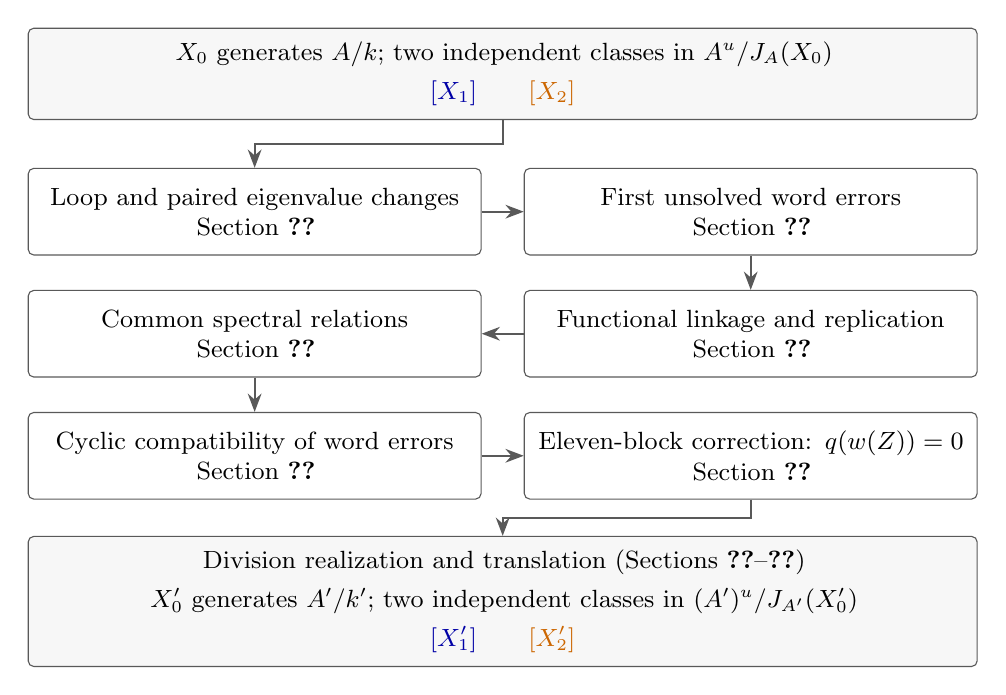
\begin{tikzpicture}[
  x=1cm,y=1cm,>=Stealth,
  every node/.style={font=\small},
  interface/.style={draw=black!65,rounded corners=2pt,align=center,
    text width=54mm,minimum height=11mm,inner sep=5pt},
  endpoint/.style={interface,text width=117mm,fill=black!3},
  flow/.style={draw=black!65,->,line width=.8pt}
]
  \node[endpoint] (input) at (0,0)
    {$X_0$ generates $A/k$; two independent classes in $A^u/J_A(X_0)$\\[3pt]
     \textcolor{blue!65!black}{$[X_1]$}\qquad
     \textcolor{orange!80!black}{$[X_2]$}};
  \node[interface] (responses) at (-3.15,-1.75)
    {Loop and paired eigenvalue changes\\
     Section~\ref{sec:responses}};
  \node[interface] (errors) at (3.15,-1.75)
    {First unsolved word errors\\
     Section~\ref{sec:word-transfer}};
  \node[interface] (linkage) at (3.15,-3.3)
    {Functional linkage and replication\\
     Section~\ref{sec:linkage-replication}};
  \node[interface] (relations) at (-3.15,-3.3)
    {Common spectral relations\\
     Section~\ref{sec:global-defect}};
  \node[interface] (cyclic) at (-3.15,-4.85)
    {Cyclic compatibility of word errors\\
     Section~\ref{sec:cyclic-obstructions}};
  \node[interface] (correction) at (3.15,-4.85)
    {Eleven-block correction: $q(w(Z))=0$\\
     Section~\ref{sec:free-correction}};
  \node[endpoint] (output) at (0,-6.7)
    {Division realization and translation
     (Sections~\ref{sec:division-realization}--\ref{sec:generation})\\[3pt]
     $X'_0$ generates $A'/k'$; two independent classes in
     $(A')^u/J_{A'}(X'_0)$\\[3pt]
     \textcolor{blue!65!black}{$[X'_1]$}\qquad
     \textcolor{orange!80!black}{$[X'_2]$}};
  \draw[flow] (input.south) -- ++(0,-.3) -| (responses.north);
  \draw[flow] (responses.east) -- (errors.west);
  \draw[flow] (errors.south) -- (linkage.north);
  \draw[flow] (linkage.west) -- (relations.east);
  \draw[flow] (relations.south) -- (cyclic.north);
  \draw[flow] (cyclic.east) -- (correction.west);
  \coordinate (outputbend) at ($(correction.south)!0.5!(output.north)$);
  \draw[flow] (correction.south) |- (outputbend) -| (output.north);
\end{tikzpicture}

\caption{The spectral case of Theorem~\ref{thm:lifting}.
The two displayed classes at each end are linearly independent in the
indicated quotient. The middle boxes describe the matrix calculation:
allowable eigenvalue changes control the first unsolved word errors,
and the cyclic relations are precisely the obstructions to correction.
Realization and translation return a generating tuple over a division
algebra of strictly larger degree. If $w$ already satisfies the minimal
polynomial of $w(0)$, the middle spectral correction is omitted, but
realization and translation remain necessary. No embedding tower of
the successive division algebras is asserted.}
\label{fig:response-interfaces}
\end{figure}
\clearpage

\section{The countable construction and the actual center}
\label{sec:countable-construction}

We now apply Theorem~\ref{thm:lifting} repeatedly.  Recall its
full conclusion: from a finite-dimensional central division algebra $A/k$
and a tuple of free series $X$ whose constant term generates $A$ and whose
two linear coefficients are independent modulo inner directions, it
produces such a tuple over a countable extension $k'$ and a central
division algebra of strictly larger degree.  It preserves every old
polynomial identity and gives a monic algebraic relation for any chosen
series $w$.  The countability, generation, and two-direction conclusions
are all needed to iterate this theorem.

The resulting division algebras need not embed in one another.  We use
an ultraproduct to retain their polynomial relations, and then prove
separately that the resulting algebra has infinite dimension over its
actual center.

\subsection{Scheduling all polynomial expressions}

Start with
\[
 k_0=\overline{\mathbb Q},\qquad A_0=k_0,\qquad
 X^{(0)}=(z_1,z_2).
\]
Its constant pair $(0,0)$ generates $k_0$ as a unital $k_0$-algebra.
The inner-direction space is zero, and its two linear coefficients
$(1,0)$ and $(0,1)$ are independent.  Thus it satisfies the hypotheses
of Theorem~\ref{thm:lifting}.

Inductively we obtain countable fields
\[
 k_0\subseteq k_1\subseteq k_2\subseteq\cdots,
\]
finite-dimensional central division algebras $A_i/k_i$ of strictly
increasing degrees, and pairs
\[
 X^{(i)}\in A_i\langle\!\langle z_1,z_2\rangle\!\rangle^2
\]
satisfying the same generation and transverse-independence hypotheses.
Write $(x_i,y_i)=X^{(i)}_0$ for the constant pair; in particular,
\begin{equation}
 A_i=k_i[x_i,y_i].
 \label{eq:stage-generation}
\end{equation}

Here is a schedule that ensures algebraicity of every expression
needed in the limit.  When $k_i$ has been constructed, enumerate the
countable set $k_i\langle x,y\rangle$ as
$(p_{i,j})_{j\geq0}$.  Enumerate the pairs $(i,j)\in\mathbb N^2$ by
increasing $i+j$, in a fixed order within each diagonal.  If $(i_n,j_n)$
is the $n$th pair, beginning at $n=0$, then $i_n\leq n$.
At stage $n$, apply the lifting theorem to
\[
 w=p_{i_n,j_n}(X^{(n)}).
\]
This expression is defined over $k_n$, since $k_{i_n}\subseteq k_n$.
The identity $w-p_{i_n,j_n}(X^{(n)})=0$ is preserved, so the new relation
for the lifted $w$ gives a nonzero monic polynomial
\[
 q_{i_n,j_n}(t)\in k_{n+1}[t]
\]
such that
\begin{equation}
 q_{i_n,j_n}\bigl(p_{i_n,j_n}(X^{(n+1)})\bigr)=0.
 \label{eq:retained-formal-relation}
\end{equation}
Every later lifting preserves this polynomial identity, now regarded
over its coefficient field $k_{n+1}$.  Taking constant terms shows that
the corresponding identity holds at $(x_h,y_h)$ for every $h\geq n+1$.
Each polynomial over each $k_i$ is treated at a finite stage.

\subsection{A two-generated algebraic division ring}

Fix a nonprincipal ultrafilter $\mathcal U$ on $\mathbb N$ and form
(see \cite{Keisler2010} for the general construction)
\[
 \mathcal D=\prod_{i\geq0} A_i\big/\mathcal U.
\]
Here two sequences represent the same element when their equality set
belongs to $\mathcal U$.  This is a division ring: a nonzero class has
nonzero coordinates on a set in $\mathcal U$, and taking their
coordinatewise inverses on that set gives its inverse.

Put $k_\infty=\bigcup_i k_i$.  An element $c\in k_j$ determines a class
in $\mathcal D$ by taking its image in the central field $k_i\subset A_i$
for $i\geq j$ and choosing arbitrary coordinates at the finitely many
earlier indices.  These classes are independent of the early choices
and of $j$.  They define a central field embedding
\[
 k_\infty\hookrightarrow\mathcal D:
\]
the field operations agree at every sufficiently large index, and a
nonzero field element stays nonzero at all those indices.  This
construction uses only the inclusions of coefficient fields; it does
not require embeddings between the algebras $A_i$.

Let
\[
 x=[(x_i)_i],\qquad y=[(y_i)_i],\qquad
 R=k_\infty[x,y]\subseteq\mathcal D.
\]
Every $r\in R$ has the form $p(x,y)$ for some
$p\in k_j\langle x,y\rangle$.  The schedule and
\eqref{eq:retained-formal-relation} provide a nonzero monic polynomial
$q\in k_h[t]$, for a suitable $h$, such that
$q(p(x_i,y_i))=0$ at every sufficiently large index.  Therefore
$q(r)=0$ in $\mathcal D$.  Every element of $R$ is algebraic over
$k_\infty$.

This already makes $R$ a division ring.  For $0\ne r\in R$, choose a
nonzero relation of least degree
\[
 a_0+a_1r+\cdots+a_nr^n=0,
 \qquad a_j\in k_\infty.
\]
Its constant coefficient is nonzero: otherwise multiplication by
$r^{-1}$ in the ambient division ring $\mathcal D$ would give a shorter
relation.  Consequently
\[
 r^{-1}=-a_0^{-1}(a_1+a_2r+\cdots+a_nr^{n-1})\in R.
\]
Since $k_\infty$ is countable and $R$ is generated by two elements as an
algebra, $R$ is countable.  Its characteristic is zero.

\subsection{Infinite dimension and passage to the center}

We first prove
\begin{equation}
 [R:k_\infty]=\infty.
 \label{eq:infinite-auxiliary-dimension}
\end{equation}
For each $i$ and $\ell\geq0$, let $V_{i,\ell}$ be the $k_i$-span of the
words in $x_i,y_i$ of length at most $\ell$, including the empty word
$1$.  If $V_{i,\ell}=V_{i,\ell+1}$, then $V_{i,\ell}$ is stable under
right multiplication by $x_i$ and $y_i$ and contains every word.
By \eqref{eq:stage-generation}, it equals $A_i$.  Until this happens,
the dimensions increase strictly, starting from $1$.

Fix $\ell$.  The dimensions $[A_i:k_i]$ tend to infinity, so
\[
 \dim_{k_i}V_{i,\ell}\geq\ell+1
\]
for every sufficiently large $i$.  There are only finitely many
subsets of size $\ell+1$ in the finite list of words of length at most
$\ell$.  The ultrafilter therefore selects one fixed subset
$w_0,\ldots,w_\ell$ that is linearly independent at a set of stages
belonging to $\mathcal U$.

These same words are independent over the embedded $k_\infty$ in $R$.
Indeed, the coefficients of a putative relation
\[
 \sum_{j=0}^{\ell} c_j w_j(x,y)=0
\]
all belong to one field $k_h$.  Equality in the ultraproduct holds on
a set in $\mathcal U$.  Intersecting it with the independence set and
the tail $i\geq h$ gives a nonempty set where stage independence
forces every $c_j$ to vanish.  Thus $R$ has arbitrarily large finite
linearly independent sets, proving
\eqref{eq:infinite-auxiliary-dimension}.

Finally let $F=Z(R)$ be the actual center.  It contains $k_\infty$ and
is algebraic over $k_\infty$, since every element of $R$ is.  In
particular, every element of $R$ is algebraic over $F$.  Also
\[
 R=k_\infty[x,y]=F[x,y]=F(x,y),
\]
because $F\subseteq R$ and $R$ is already a division ring.

We use finite descent of the multiplication table and generator
coordinates; compare the proof of the local-finiteness criterion in
\cite[Section~4]{DeoBienHai2019}. Suppose, for a contradiction, that
$[R:F]=n<\infty$. Choose an
$F$-basis $b_1=1,b_2,\ldots,b_n$ of $R$, and write
\[
 b_i b_j=\sum_{h=1}^n c_{ijh}b_h,
 \qquad
 x=\sum_{h=1}^n u_hb_h,
 \qquad
 y=\sum_{h=1}^n v_hb_h,
\]
with all coefficients in $F$.  Let $E$ be the subfield of $F$
generated over $k_\infty$ by these finitely many coefficients.
Algebraicity gives $[E:k_\infty]<\infty$.  The space
\[
 B=\sum_{h=1}^n E b_h
\]
contains $1,x,y$ and is closed under multiplication by the displayed
structure constants.  It is therefore a $k_\infty$-subalgebra of $R$
containing $k_\infty[x,y]=R$, so $B=R$.  This implies
\[
 [R:k_\infty]\leq n[E:k_\infty]<\infty,
\]
contrary to \eqref{eq:infinite-auxiliary-dimension}.

Thus the countable characteristic-zero division ring $D=R$ is
algebraic over its actual center $F$, while
\[
 D=F[x,y]=F(x,y),\qquad [D:F]=\infty.
\]
The finite set $\{x,y\}$ witnesses the failure of local finiteness.

This proves Theorem~\ref{thm:main}, subject only to Theorem~\ref{thm:lifting},
which we now prove.

\section{Formal evaluations and generic spectra}\label{sec:formal-generic}

We begin the proof of Theorem~\ref{thm:lifting} by constructing a
substitution $Z=(Z_1,Z_2)$ for the two free letters. Its coefficients will commute
with the old algebra $A$, so applying it to $(X,w)$ preserves their
polynomial identities. The matrix calculation focuses on $w$;
Sections~\ref{sec:division-realization} and~\ref{sec:generation}
realize the substitution in a division algebra of larger degree and
restore generation and both transverse directions for $X(Z)$.

Throughout the lifting argument, $k$ is a field of characteristic zero
containing all roots of unity, $A$ is a central division algebra of degree
$d$ over $k$, and
\[
 w\in A\langle\!\langle z_1,z_2\rangle\!\rangle.
\]
The letters commute with $A$, but not with each other.  Thus an element
is a family $(a_\omega)_\omega$ indexed by finite words, written
$\sum_\omega a_\omega z^\omega$, and multiplication uses concatenation
of words.  Fix an algebraic closure $K$ of $k$ and a splitting
$A\otimes_k K\simeq M_d(K)$; this uses the splitting and
scalar-extension properties of central simple algebras
\cite[Chapter~IV, Example~2.14(a) and Proposition~2.15]{MilneCFT}.

If $P=(P_1,P_2)$ is a pair of $n\times n$ indeterminate matrices, put
\[
 W_n(P)=\sum_\omega a_\omega\otimes P^\omega
       \in M_{dn}(K[[P]]).
\]
Here $K[[P]]$ is the ordinary commutative power series ring in the
$2n^2$ entries.  We omit the subscript $n$ when the size is clear.
The coefficient matrices act on the first tensor factor.  In
particular, every input arrow between blocks is a pair of scalar
matrices acting on the second factor.  It is not an arbitrary pair of
matrices on both factors.

In the spectral case we seek a substitution $Z=(Z_1,Z_2)$, with
constant term $R$, for which $W(Z)$ is conjugate to a split semisimple
constant output $W(R)$. If $\Lambda$ is the set of distinct eigenvalues
of $W(R)$, this gives
\[
 q(W(Z))=0,\qquad q(t)=\prod_{\lambda\in\Lambda}(t-\lambda).
\]
The division realization will identify $q$ with the minimal polynomial
over its central coefficient field. If $w$ already satisfies the
minimal polynomial of $w(0)$, substitution retains that relation and
the spectral correction is unnecessary.

For the spectral construction, we will find matrix sizes with a common
eigenvalue multiplicity, disjoint spectra at independent inputs, and
scalar spectral blocks under commuting Taylor perturbations. These
properties will make the eigenvalue responses of
Section~\ref{sec:responses} well-defined. We first specify the
evaluations and specializations used to establish them and to evaluate
triangular auxiliary inputs later.

\subsection{Convergence and specialization}\label{subsec:formal-conventions}

Let $E$ be a complete discretely valued field containing $K$, with
valuation $v$, such that $v(c)=0$ for $c\in K^\times$.  We use
$E=C((\varepsilon))$, or a finite extension of such a field, and
normalize $v(\varepsilon)=1$.  Matrix valuations mean the minimum of
the entry valuations.  A matrix is \emph{small} if this minimum is
positive.  A small generic point is
$P=\varepsilon P^\circ$, where all entries of $P^\circ$ are
algebraically independent over the previously specified constant
field.  Several independent points can use the same $\varepsilon$.

The finite extensions used to split spectra are separable in
characteristic zero. The valuation extends to each such extension,
which remains complete and discretely valued
\cite[Theorem~7.38 and Remark~7.43]{MilneANT}; with the normalization
$v(\varepsilon)=1$, its value group may be $\frac1e\mathbb Z$ for a
positive integer $e$.

\begin{lemma}[Admissible evaluations]\label{lem:admissible-evaluation}
Suppose a constant input pair $R$ is block upper triangular with $b$
blocks and small diagonal blocks.  Its strictly upper blocks may have
arbitrary entries in $E$.  Let $H$ be a matrix pair of formal series
of positive order in finitely many commuting or free variables.
Then $W(R+H)$ is defined coefficientwise by convergent sums in $E$.
The same assertion holds for products, finite determinants, and
derivatives of fixed order of finitely many such entry series.

These evaluations preserve formal entry identities.  They also
remain valid coefficientwise in an additional parameter $\eta$ if
the diagonal blocks have entries in $E[[\eta]]$ with small constant
terms, while the strictly upper blocks and the coefficients of $H$
have entries in $E((\eta))$.
\end{lemma}

\begin{proof}
Fix a coefficient of degree $r$ in the variables of $H$.  An input
path contributing to this coefficient uses at most $r$ positive-order
terms of $H$.  Between these insertions it follows the constant upper
triangular pair.  In each of the at most $r+1$ resulting intervals,
there are at most $b-1$ strictly upper steps.  Thus at most
$(r+1)(b-1)$ constant factors are strictly upper.  All remaining
constant factors come from small diagonal blocks.

Only finitely many coefficients of $H$ can occur at the chosen degree.
Their valuations, and those of the finitely many strictly upper
blocks, have a common lower bound.  If the original word has length
$L$, its contribution consequently has valuation at least
$cL-C_r$, where $c>0$ and $C_r$ is independent of the word.  There
are finitely many words of each length, so the sum converges.  The
same estimate applies after inserting the finitely many extra factors
needed for a product or a derivative of fixed order.  Completeness
allows regrouping of these sums, proving compatibility with
multiplication and with identities.

For the last assertion, first fix both the degree $r$ in $H$ and an
$\eta$-coefficient.  The bounded number of strictly upper steps and
of $H$-insertions bounds their total negative $\eta$-order.  Hence
only a bounded number of positive-order diagonal $\eta$-terms can
contribute, and only finitely many of their coefficients are used.
Every other factor is a small constant diagonal term.  The preceding
valuation estimate therefore applies again.  The resulting assertion
is coefficientwise; no interchange of the two Laurent topologies is
being asserted.
\end{proof}

We will use inverses of finite matrices as rational operations after
evaluation.  The following elementary distinction is important.
Although $(\varepsilon-Q)^{-1}$ has a formal expansion at $Q=0$ over
$E$, that expansion need not converge after $Q=\varepsilon Q^\circ$.
Accordingly, when transferring an identity involving an inverse, we
first multiply by its determinant.  We evaluate the resulting
numerator by Lemma~\ref{lem:admissible-evaluation}, and divide only
when the evaluated determinant is nonzero.  Formal inverse expansions
are used to define coefficients; they are not presumed to converge at
every subsequent specialization.

\begin{lemma}[Detection by independent residues]\label{lem:generic-detection}
Let
\[
 F(Q)=\sum_\alpha c_\alpha Q^\alpha\in E[[Q_1,\ldots,Q_N]],
 \qquad \inf_\alpha v(c_\alpha)>-\infty.
\]
Adjoin elements $Q_1^\circ,\ldots,Q_N^\circ$ whose residues are
algebraically independent over the residue field of $E$, and complete
with respect to the extended valuation.  Then
$F(\varepsilon Q^\circ)$ is defined, and is nonzero whenever $F$ is
nonzero.
\end{lemma}

\begin{proof}
The valuations $v(c_\alpha)+|\alpha|$ tend uniformly to infinity
with $|\alpha|$.  Their least value is therefore attained by a
nonempty finite set of monomials.  After scaling to this valuation,
the residue of their sum is a nonzero polynomial in the independent
residues of the $Q_j^\circ$.  This proves both assertions.
\end{proof}

In applications, the coefficients of a cleared numerator are finite
sums of products of base-point scalars and matrix-entry series.
The path estimate gives a uniform valuation bound in the auxiliary
coordinates.  Lemma~\ref{lem:generic-detection} therefore identifies
formal identities in these coordinates with identities at independent
small generic points.  The base-point valued field is constructed
first; the auxiliary residues are adjoined afterward.  This order
keeps their independence valid even after the base spectrum has been
split.  The argument can be applied separately at each Taylor degree.

We record two further field conventions.  Evaluation
\[
 K[[P]]\longrightarrow C(P^\circ)((\varepsilon)),
 \qquad P\longmapsto\varepsilon P^\circ,
\]
is injective, by homogeneous degree or by
Lemma~\ref{lem:generic-detection}.  It extends to the fraction field,
and a finite splitting field embeds into a finite algebraic extension
of the target.  Also, if $R$ is a small constant pair, then
\begin{equation}
K[[P]]\longrightarrow E[[\Delta]],\qquad P\longmapsto R+\Delta
 \label{eq:generic-taylor-embedding}
\end{equation}
is injective: reduction modulo the valuation ideal sends the image of
$f$ to $f(\Delta)$.  We use this observation for small block diagonal
$R$.  Denominators in the fraction field remain nonzero, so the map
extends to fraction fields.

Finally, the Taylor substitution $P\mapsto P+\eta v$ maps
$\operatorname{Frac}K[[P]]$ into
$\operatorname{Frac}K[[P]][[\eta]]$, with reduction the identity.
It extends to a finite separable extension $\Omega$ with values in
$\Omega[[\eta]]$: choose a primitive element and lift its defining
equation using its nonzero derivative.  The lift reducing to the
chosen primitive element is unique, by coefficient recursion.  This
convention lets us move a base point while retaining its labeled
eigenvalue branches.

\subsection{Generic division evaluations}\label{subsec:generic-division}

Generic matrix evaluations have a useful divisibility property for
their eigenvalue multiplicities.  We obtain it by first evaluating
inside a division algebra.

For $n\ge1$, choose independent central variables $\alpha,\beta$
and a primitive $n$th root of unity $\zeta_n\in k$.  Over
$k_0=k(\alpha,\beta)$ let $B_n$ be generated by $x,y$ with
\[
 x^n=\alpha,\qquad y^n=\beta,\qquad yx=\zeta_nxy.
\]
For $n=1$ this means $B_1=k_0$.  The reduced monomials
$x^iy^j$, $0\le i,j<n$, form a basis.  Indeed they span by the
relations, and after adjoining $n$th roots of $\alpha$ and $\beta$
their clock-and-shift matrices are linearly independent.  These
matrices span $M_n$, so $B_n$ is central simple of degree $n$.
This is the standard symbol construction
\cite[Corollary~2.5.5(1)]{GilleSzamuely2006}, with the inverse
root of unity for our convention.

\begin{lemma}\label{lem:symbol-division}
The central simple algebra $A\otimes_k B_n$ is division.  Its pure
rational scalar extensions and its central Laurent series extensions
are division as well.
\end{lemma}

\begin{proof}
Start with $A((x))$, where $x$ commutes with $A$, and let $\sigma$
fix $A$ and send $x$ to $\zeta_nx$.  The skew Laurent series ring
$A((x))((y;\sigma))$, with $ya=\sigma(a)y$, is a division ring by
the leading-coefficient construction of inverses.  The elements
$x^n,y^n$ are central and algebraically independent.  The defining
relations give a unital map of $A\otimes_k B_n$ into this division
ring.  Central simplicity makes the map injective.  A finite
dimensional domain over a field is division, since multiplication by
a nonzero element is an injective and hence surjective linear map.

For a central division algebra $D/F$, the rational extension $D(t)$
embeds in the division ring $D((t))$.  Iterating proves the rational
assertion.  Because $D$ has a finite $F$-basis,
$D\otimes_F F((\varepsilon))=D((\varepsilon))$, which is again
division by leading coefficients.
\end{proof}

Choose a basis $b_1,\ldots,b_{n^2}$ of $B_n$, and let
$c_{ij}$, $i=1,2$, $j=1,\ldots,n^2$, be independent variables.
Evaluate $w$ at
\[
 P_i=\varepsilon\sum_j c_{ij}b_j.
\]
This gives an element of a central division algebra of degree $dn$
over
\[
 F_n=k(\alpha,\beta,(c_{ij}))((\varepsilon)).
\]
After splitting $A$ and $B_n$ by constants independent of the $c_{ij}$,
the $b_j$ become a basis of $M_n$.  The change from the $c_{ij}$ to
the entries of $P_i/\varepsilon$ is therefore an invertible linear
change of independent coordinates.  The resulting evaluation is a
small generic scalar matrix evaluation in the sense fixed above.

Let $e_n$ denote the minimal-polynomial degree of this element.  Its
minimal polynomial is irreducible and separable over $F_n$.
Consequently $W(P)$ is semisimple over a splitting field, and every
distinct root has the same multiplicity
\begin{equation}
t_n=\frac{dn}{e_n}.
 \label{eq:generic-multiplicity}
\end{equation}
For completeness, if $D/F$ has degree $N$ and $a\in D$ has minimal
polynomial $q$ of degree $e$, then left multiplication by $a$ has
characteristic polynomial $q^{N^2/e}$: view $D$ as a vector space
over $F[a]$.  After splitting $D=M_N$, left multiplication acts by
the matrix $a$ on each of its $N$ columns.  Its characteristic
polynomial is therefore the $N$th power of the matrix characteristic
polynomial.  Comparing root multiplicities gives $N/e$ in the
matrix representation.  This also proves that $N/e$ is an integer.

Linear independence of $1,a,\ldots,a^{e-1}$ is preserved by field
extension.  Thus the same $e_n,t_n$ describe $W(P)$ over a splitting
field of $\operatorname{Frac}K[[P]]$.

\subsection{Nonconstant roots and stable multiplicity}
\label{subsec:stable-multiplicity}

Let $q_0$ be the minimal polynomial of $w(0)$ over $k$.  If
$q_0(w)=0$ as a free series, the subsequent spectral construction is
unnecessary; the unconstrained case of the lifting argument will use
this existing relation.  In the rest of this section assume
$q_0(w)\ne0$.

A nonzero homogeneous part of $q_0(w)$ is detected by scalar matrices
of every sufficiently large size.  To see this, choose a word of
length $L$ with nonzero coefficient and use a path of $L+1$ vertices,
placing its successive letters on the consecutive matrix-unit
arrows.  The $(1,L+1)$ entry detects precisely that coefficient.
Padding by zero blocks works for all larger sizes.  It follows that
$q_0(W(P))\ne0$ at every generic size $n\ge n_0$, for some $n_0$.

\begin{lemma}\label{lem:nonconstant-roots}
For $n\ge n_0$, every distinct generic eigenvalue of $W(P)$ has a
nonzero differential in the input entries.  Independent small generic
points of sizes at least $n_0$ have disjoint spectra.  Their spectra
also avoid the constant spectrum of $w(0)$.
\end{lemma}

\begin{proof}
Use the division evaluation over $F_n$.  Each derivation
$\partial/\partial c_{ij}$ acts coefficientwise on Laurent series
and extends uniquely to algebraic extensions in characteristic zero.
Uniqueness implies that it commutes with automorphisms of a splitting
field over $F_n$.  If all these derivations killed one root, they
would kill all its Galois conjugates.  Irreducibility makes these all
the distinct roots.  Thus every coefficient of the reduced
characteristic polynomial would have all its input derivatives zero.

The coefficient of $\varepsilon^r$ in such a characteristic
coefficient is a homogeneous polynomial of degree $r$ in the
$c_{ij}$.  In characteristic zero a polynomial whose partial
derivatives all vanish is constant.  All terms of positive
$\varepsilon$-degree therefore vanish.  The characteristic polynomial
is the characteristic polynomial of $w(0)$.  Semisimplicity then
implies $q_0(W(P))=0$, a contradiction.

Splitting $A,B_n$ uses constants independent of the inputs.  The
invertible basis change described above, together with the nonzero
factor $\varepsilon$, transports the differential assertion to
ordinary matrix-entry coordinates.  For independent points $P,Q$,
derivations in the $P$-coordinates kill the roots belonging to $Q$.
They cannot kill a root belonging to $P$.  No root can therefore
belong to both spectra.  The same argument excludes a constant root.
\end{proof}

Choose $p\ge n_0$ for which the positive integer $t_p$ is minimal
among all $t_n$, $n\ge n_0$, and put
\[
 t=t_p,\qquad \mathcal S=\{pN:N\ge1\}.
\]

\begin{lemma}\label{lem:stable-multiplicity}
For every $N\ge1$,
\[
 t_{pN}=t,\qquad e_{pN}=Ne_p.
\]
\end{lemma}

\begin{proof}
Specialize a size-$pN$ point to a diagonal sum of $N$ independent
size-$p$ points.  Lemma~\ref{lem:nonconstant-roots} gives $Ne_p$
distinct eigenvalues there.  The generic bound on minimal-polynomial
degree survives this specialization: it is expressed by the vanishing
of all $(e_{pN}+1)$-minors of the matrix whose columns are the
vectorizations of $1,W,\ldots,W^{e_{pN}}$.  These are formal entry
identities covered by Lemma~\ref{lem:admissible-evaluation}.
Consequently $e_{pN}\ge Ne_p$.  Minimality of $t$ gives the opposite
inequality,
$e_{pN}=dpN/t_{pN}\le dpN/t=Ne_p$.
\end{proof}

We henceforth use sizes in $\mathcal S$.  At size $n$, the minimal
polynomial always has degree at most $e_n=dn/t$ at every admissible
specialization.  The following consequence controls all commuting
Taylor deformations used below.

\begin{lemma}[Scalar branches at maximal root count]
\label{lem:scalar-branches}
Let $V(T)$ be a matrix over a commuting formal Taylor ring $E[[T]]$.
Suppose $V(0)$ is split semisimple with $e$ distinct eigenvalues and
the minimal-polynomial degree of $V(T)$ over
$\operatorname{Frac}E[[T]]$ is at most $e$.  Then a formal change of
basis reducing to the identity separates $V(T)$ into $e$ scalar
blocks.  The sizes of these blocks are their multiplicities at
$T=0$.
\end{lemma}

\begin{proof}
Use the eigenspace decomposition at zero.  Off-diagonal blocks can be
removed recursively in total Taylor degree: the equation for the
block between eigenvalues $\lambda_i,\lambda_j$ is multiplication
by $\lambda_i-\lambda_j$, a nonzero scalar.  We obtain blocks
$V_i(T)$ reducing to $\lambda_i I$.  Their characteristic polynomials
have pairwise unit resultants, because their reductions have different
roots.  Their minimal polynomials over the Taylor fraction field are
therefore pairwise coprime.  The minimal-polynomial degree of their
direct sum is the sum of their degrees.  There are $e$ nonempty
blocks and the total degree is at most $e$, so every block has
minimal-polynomial degree one.  Each $V_i(T)$ is scalar.  Its scalar
entry belongs to $E[[T]]$, since the block entries do.
\end{proof}

In particular, the roots at a small semisimple point with $e_n$
distinct roots have labeled scalar Taylor branches.  The splitting
field of the generic point embeds in their Taylor fraction field by
\eqref{eq:generic-taylor-embedding}; a labeling is chosen by reduction
to the roots at the base.

Let $\rho_n$ be the generic rank of the input Jacobian of
\[
 \operatorname{tr}W,\operatorname{tr}W^2,\ldots,
 \operatorname{tr}W^{dn}.
\]
Its minors are formal entry identities, so $\rho_n$ bounds the
corresponding specialized ranks.  At a maximal-root-count point the
scalar branches satisfy
\[
 d\operatorname{tr}W^j
   =jt\sum_{h=1}^{e_n}\lambda_h^{j-1}\,d\lambda_h.
\]
The first $e_n$ rows give an invertible Vandermonde matrix.  Hence
the trace Jacobian and the eigenvalue Jacobian have the same rank
there, including over a commuting Taylor fraction field.  We have
therefore obtained both ingredients needed for the response
calculations: scalar branches and specialization-stable rank bounds.

\section{The space of eigenvalue responses}\label{sec:responses}

Fix a size $n\in\mathcal S$, a generic input pair $P$, and a splitting
field $\Omega_P$ of $W(P)$ over $\operatorname{Frac}K[[P]]$.
Write its distinct roots as $\lambda_h$, with spectral projections
$\pi_h$, $1\le h\le e_n$.  Each projection has rank $t$.
We also use these data after embedding into the valued fields of
Section~\ref{sec:formal-generic}.

We seek the possible leading changes of the eigenvalues at $P$.
Besides varying $P$ itself, we allow an excursion through another
input block and a return to $P$.  Their linear span will determine
which eigenvalues can be varied independently.

\subsection{Loop and paired responses}\label{subsec:response-formulas}

Upper triangular block evaluations are also the basic mechanism of
noncommutative difference-differential calculus; see
\cite[Proposition~2.2 and Theorem~3.11]{KaliuzhnyiVerbovetskyiVinnikov2014}.
Here the admissible evaluations of Section~\ref{sec:formal-generic}
let us extract scalar eigenvalue responses from those block calculations.

For a perturbation $\mathcal W$ of $W(P)$, put $\pi=\pi_h$,
$\bar\pi=1-\pi$, and
\[
 C_h(\mathcal W)=\bar\pi(\mathcal W-\lambda_h)\bar\pi.
\]
This operator acts on the complementary space. Its constant term is
invertible, so its inverse has a unique expansion in either commuting
or free formal parameters. Define the fixed-root Schur expression by
\begin{equation}
S_h(\mathcal W)=
 \pi(\mathcal W-\lambda_h)\pi
 -\pi\mathcal W\bar\pi
  C_h(\mathcal W)^{-1}
  \bar\pi\mathcal W\pi.
 \label{eq:fixed-schur}
\end{equation}
This expression records the obstruction to keeping the root $\lambda_h$
fixed. For $u$ in the image of $\pi$, the vector
\[
 u-C_h(\mathcal W)^{-1}\bar\pi\mathcal W\pi u
\]
is the unique vector projecting to $u$ whose complementary component
under $\mathcal W-\lambda_h$ vanishes. Its remaining component is
$S_h(\mathcal W)u$. Thus $S_h(\mathcal W)=0$ means that the fixed-root
kernel is a graph over the original eigenspace.

When the constant output is split semisimple and these equations are
imposed for every one of its distinct roots, the kernel graphs combine
into a formal change of basis. The output remains conjugate to its
constant term and satisfies that constant term's minimal polynomial.
Lemma~\ref{lem:schur-polynomial} proves the equivalence with the
polynomial identity at every finite word order.

The same Schur expression is defined near $\operatorname{diag}(P,C_0)$
if $\lambda_h$ is absent from $W(C_0)$, embedding $\pi_h$ at the $P$
block. In this use, equations indexed by labels at $P$ record those
fixed roots only.

For a loop direction $Y=(Y_1,Y_2)$ at $P$, define the scalar
$D_h(P;Y)$ by
\begin{equation}
\pi_h W'_P(Y)\pi_h=D_h(P;Y)\pi_h.
 \label{eq:loop-response}
\end{equation}
This compression is scalar: apply Lemma~\ref{lem:scalar-branches}
to the commuting deformation $P+xY$ and take its first coefficient.
Equivalently, $D_h(P;Y)$ is the differential of the branch
$\lambda_h$ in direction $Y$.  By
Lemma~\ref{lem:nonconstant-roots}, each of these linear functionals is
nonzero.  Because $K$ is infinite, we can choose a constant direction
$v$ over $K$ with
\begin{equation}
D_h(P;v)\ne0\qquad(1\le h\le e_n).
 \label{eq:nonzero-direction}
\end{equation}
Indeed the forbidden directions form a finite union of proper
$K$-linear subspaces, even though their defining coefficients belong
to $\Omega_P$.

Let $Q$ be an independent generic point of size $n'\in\mathcal S$.
Let $U$ be an input arrow $P\leftarrow Q$ and $V$ an input arrow
$Q\leftarrow P$; each is a pair of rectangular scalar matrices.
Form the triangular input pair
\[
 T=\begin{pmatrix}P&U&0\\0&Q&V\\0&0&P\end{pmatrix}.
\]
Set
\begin{equation}
M_h(P,Q;U,V)=\pi_h\left(
 W(T)_{13}
 -W(T)_{12}(W(Q)-\lambda_h)^{-1}W(T)_{23}
 \right)\pi_h.
 \label{eq:paired-response}
\end{equation}
Block paths show that this is bilinear in $U,V$.  The inverse exists
because the spectra at independent points are disjoint.

\begin{lemma}\label{lem:paired-scalar}
There is a scalar $m_h(P,Q;U,V)$ such that
\[
 M_h(P,Q;U,V)=m_h(P,Q;U,V)\pi_h.
\]
It is the coefficient of $xy$ in the branch reducing to $\lambda_h$
for the commuting input deformation
\[
 \begin{pmatrix}P&xU\\yV&Q\end{pmatrix}.
\]
The same assertion holds at an admissible specialized pair whose
spectra are disjoint and whose combined output is split semisimple
with the maximal number $e_{n+n'}$ of distinct roots.
\end{lemma}

\begin{proof}
At $x=y=0$, disjointness and Lemma~\ref{lem:stable-multiplicity}
give $e_n+e_{n'}=e_{n+n'}$ roots.  Thus
Lemma~\ref{lem:scalar-branches} applies.  Either arrow alone leaves
the spectrum unchanged, so the chosen branch has no terms depending
on $x$ alone or on $y$ alone.

Compute the $xy$ coefficient of its fixed-root Schur expression.
The direct return from $P$ through $Q$ gives $W(T)_{13}$.  Eliminating
the $Q$ block gives the second term in
\eqref{eq:paired-response}.  The other eigenspaces in the $P$ block
give no further term of this order: their couplings to $\pi_h$ have
zero constant term and no first-order term under these off-diagonal
input perturbations.  Replacing the fixed root by the scalar branch
subtracts its $xy$ coefficient times $\pi_h$.  The resulting Schur
expression vanishes, because the branch eigenspace projects
isomorphically to the base eigenspace.  This proves the formula.
The specialized assertion uses exactly the same argument and the
specialization-stable degree bound.
\end{proof}

\subsection{Coefficient spans and their specializations}
\label{subsec:active-space}

At $Q=0$ the matrices $W(Q)-\lambda_h$ are invertible, since no
$\lambda_h$ belongs to the spectrum of $w(0)$.  Hence
\eqref{eq:paired-response} has a formal expansion in the entries of
$Q$ over $\Omega_P$.  Define
\[
 m_h=\frac1t\operatorname{tr}M_h,
 \qquad m=(m_h)_{h=1}^{e_n},\qquad D=(D_h)_{h=1}^{e_n}.
\]
Here $D=D(P;\cdot):M_n(\Omega_P)^2\to\Omega_P^{e_n}$ is the linear
map of loop responses. Its columns are its values on the standard
coordinate directions in the two input matrices.
The scalar identity of Lemma~\ref{lem:paired-scalar} holds also for
these formal expansions, by clearing their determinants and applying
Lemma~\ref{lem:generic-detection}.

Define $\mathcal T_P\subseteq\Omega_P^{e_n}$ to be the linear span
of the columns of $D$ and of every coefficient vector of $m$, for
every allowed partner size $n'\in\mathcal S$ and every pair of
coordinate arrows $U,V$.  Write
\[
 a_n=\dim_{\Omega_P}\mathcal T_P.
\]
Although the definition permits infinitely many partner sizes and
coefficients, the ambient space is finite dimensional.

\begin{lemma}[Specialization and finite witnesses]
\label{lem:active-specialization}
The scalar identities for $M_h$ and every linear identity expressing
$m\in\mathcal T_P$ hold after any admissible specialization of the
partner input for which the required inverses exist.  For identities
on a subset of labels, only the inverses for those labels are needed.

After a field extension, the columns of $D$ and finitely many paired
responses span $\mathcal T_P$.  These responses can be taken at
independent small generic partner points, whose sizes need not be
equal.
\end{lemma}

\begin{proof}
For the first assertion, apply any $\Omega_P$-linear functional
annihilating $\mathcal T_P$ to the formal tuple $m$.  The result is
zero.  Multiply by the finitely many determinants of
$W(Q)-\lambda_h$ that occur.  The cleared expression is a finite
sum of products of base-point scalars and matrix-entry series; its
auxiliary coefficients have a uniform valuation bound.  Its formal
identity is therefore equivalent to its identity at a small generic
partner, by Lemma~\ref{lem:generic-detection}.  It persists under the
admissible specializations of Lemma~\ref{lem:admissible-evaluation}.
Divide by the specialized determinants when they are nonzero.  The
same argument, entry by entry, proves the scalar identities for
$M_h$.  It also proves the projected assertion, without introducing
any spectral labels for the partner input.

Choose finitely many coefficient vectors, together with columns of
$D$, that span $\mathcal T_P$, and select a nonzero minor witnessing
their rank.  For each column requiring a partner, use a separate set
of partner variables.  By multilinearity, the corresponding
determinant of the series columns has that nonzero minor as the
coefficient of a specified product of monomials.  It is therefore a
nonzero formal series.  Clear the column denominators.  The numerator
is still nonzero, and its coefficients are uniformly bounded below
in valuation.  Independent small generic evaluations keep this
numerator and its denominators nonzero, by
Lemma~\ref{lem:generic-detection}.  The resulting values attain the
full dimension.  The first assertion places all of them in the
extended active space.

This argument evaluates cleared numerators, not the possibly
divergent geometric expansions of their inverses.  The distinction
is precisely the one made in Section~\ref{subsec:formal-conventions}.
\end{proof}

The lemma also applies after adjoining Taylor or Laurent parameters.
One first clears determinants and then works coefficientwise as in
Lemma~\ref{lem:admissible-evaluation}.  In particular, it permits
triangular partners with repeated base blocks, provided the inverses
required for the selected target roots exist in the chosen Laurent
field.

\subsection{A partition of the eigenvalue labels}
\label{subsec:active-partition}

The active space has a stronger structure than a general linear
subspace.  Its coordinates form groups whose responses are always in
a fixed ratio.

\begin{proposition}\label{prop:active-partition}
For the direction $v$ chosen in \eqref{eq:nonzero-direction}, there
is a partition of $\{1,\ldots,e_n\}$ such that
\[
 \mathcal T_P=
 \left\{c\in\Omega_P^{e_n}:
 \frac{c_h}{D_h(P;v)}\text{ is constant on each part}\right\}.
\]
\end{proposition}

\begin{proof}
We first prove that $\mathcal T_P$ is closed under the operation
\begin{equation}
(a,b)\longmapsto
 \left(\frac{a_hb_h}{D_h(P;v)}\right)_h.
 \label{eq:weighted-product}
\end{equation}
Choose two finite spanning sets supplied by
Lemma~\ref{lem:active-specialization}, using independent partner
points for the two sets.  It suffices to prove the assertion for a
column $a$ in the first set and a column $b$ in the second, over their
joint coefficient field $E$.

Put $P'=P+\xi v$.  Use a triangular chain with endpoints $P,P$,
middle point $P'$, an optional point $Q_1$ between the first endpoint
and $P'$, and an optional point $Q_2$ between $P'$ and the last
endpoint.  A direct step represents a loop column; an excursion
through $Q_i$ represents a paired column.  Put the arrows defining
$a$ and $b$ on the successive steps, with no other input arrows.
Group the internal positions as a single partner $C(\xi)$.  Its
size belongs to $\mathcal S$.

For every target label, $W(C(\xi))-\lambda_h$ is invertible over
$E((\xi))$.  The optional blocks have spectra disjoint from $P$.
At the middle block, the branch reducing to $\lambda_h$ moves with
nonzero derivative $D_h(P;v)$; all other branches are already away
from $\lambda_h$.  Thus
\begin{equation}
\left.\xi\bigl(W(P')-\lambda_h\bigr)^{-1}\right|_{\xi=0}
   =\frac{\pi_h}{D_h(P;v)}.
 \label{eq:middle-residue}
\end{equation}
This follows directly by scalar branch separation.

By Lemma~\ref{lem:active-specialization}, the paired response through
$C(\xi)$ belongs to $\mathcal T_P\otimes E((\xi))$.  Eliminate
the optional blocks first in its Schur formula.  Triangularity means
that their elimination does not change the middle diagonal block.
All terms are regular at $\xi=0$ except the middle inverse in
\eqref{eq:middle-residue}.  The effective first-to-middle coupling,
compressed by $\pi_h$ at both ends and evaluated at zero, is
$a_h\pi_h$.  For a direct step this is
\eqref{eq:loop-response}; for an excursion it is
\eqref{eq:paired-response}.  The corresponding middle-to-last
coupling is $b_h\pi_h$.

The singular term occurs with the minus sign in the Schur
complement.  Multiplying by $\xi$ and reducing at zero therefore
gives
\[
 \left(-\frac{a_hb_h}{D_h(P;v)}\right)_h
       \in\mathcal T_P\otimes E.
\]
Taking a Laurent coefficient preserves membership in this fixed
finite dimensional space: apply its annihilating linear functionals.
Bilinearity and the two spanning sets prove closure under
\eqref{eq:weighted-product} after extension to $E$, and faithful
scalar extension proves it over $\Omega_P$.

Divide coordinates by the nowhere-zero vector $D(P;v)$.  The resulting
space $\mathcal U\subseteq\Omega_P^{e_n}$ contains $1$, since
$D(P;v)\in\mathcal T_P$, and is closed under coordinatewise
multiplication.  Declare two coordinates equivalent if every element
of $\mathcal U$ has the same value on them.  By avoiding finitely
many proper linear subspaces, choose an element of $\mathcal U$
whose values distinguish all the equivalence classes.  Lagrange
interpolation in this element gives the indicator function of each
class.  These indicators span all class-constant functions.  Thus
$\mathcal U$ is exactly that algebra of functions, proving the
proposition.
\end{proof}

We call two labels in the same part \emph{linked}.  The number of
parts is $a_n$.  Selecting one representative from each part
identifies $\mathcal T_P$ with the full coordinate space on those
representatives.  The next stage must show that these response
relations control higher-order free-letter errors, rather than only
the two elementary perturbations used to define them.

\section{Transfer of the first unsolved word coefficient}
\label{sec:word-transfer}

Our next objective is to control equations in free letters.  The first and
paired responses describe matrix perturbations with one loop or two opposite
arrows.  We show that they also contain the first unsolved coefficient of an
arbitrary free-series perturbation.  The argument unfolds a word along a
triangular chain and then replaces its internal states by a single auxiliary
partner.  The only difficulty is that this partner initially has the target
eigenvalue.  The following linear-algebra observation explains how to remove
that singularity without changing the coefficient being computed.

\begin{lemma}[An inverse between two vanishing couplings]
\label{lem:killed-pole}
Let $E$ be a field and let $M(\xi)\in\operatorname{End}_E(V)[[\xi]]$, where
$V$ is finite dimensional.  Suppose that zero is a semisimple eigenvalue of
$M_0=M(0)$, and let $\Pi$ be its spectral projection.  Suppose that
\[
 G=\Pi M'(0)\Pi\big|_{\ker M_0}
\]
is invertible.  Then $M(\xi)^{-1}$ exists over $E((\xi))$ and has a pole of
order at most one.  Let $J$ be zero on $\ker M_0$ and equal to $M_0^{-1}$ on
$\operatorname{im}M_0$.  If $L(\xi)$ and $B(\xi)$ are compatible matrix
series satisfying
\[
 L(0)\Pi=0,\qquad \Pi B(0)=0,
\]
then
\begin{equation}
\label{eq:killed-pole-limit}
 \lim_{\xi\to0}L(\xi)M(\xi)^{-1}B(\xi)=L(0)JB(0).
\end{equation}

Suppose additionally that $e$ is an idempotent, $f=1-e$,
$fM_0f$ is invertible on $fV$, and $e:\ker M_0\to eV$ is an isomorphism.
Under the same two coupling conditions,
\begin{equation}
\label{eq:fixed-complement-inverse}
 L(0)JB(0)=L(0)f(fM_0f)^{-1}fB(0).
\end{equation}
\end{lemma}

\begin{proof}
Use $V=\ker M_0\oplus\operatorname{im}M_0$.  In this decomposition
\[
 M(\xi)=
 \begin{pmatrix}
  \xi G+O(\xi^2)&O(\xi)\\
  O(\xi)&M_0|_{\operatorname{im}M_0}+O(\xi)
 \end{pmatrix}.
\]
The lower-right block is invertible and the Schur complement of that block
is $\xi G+O(\xi^2)$.  The upper-left block of $M(\xi)^{-1}$ is consequently
$\xi^{-1}G^{-1}+O(1)$; its off-diagonal blocks are bounded; and its
lower-right block tends to $M_0^{-1}|_{\operatorname{im}M_0}$.
The kernel components of both couplings are $O(\xi)$.  Multiplying these
four blocks proves \eqref{eq:killed-pole-limit}.

For the second assertion, write $b=B(0)u$.  The condition $\Pi b=0$ places
$b$ in $\operatorname{im}M_0$.  Solutions of $M_0x=b$ differ by
$\ker M_0$.  Since projection to $eV$ is an isomorphism on that kernel,
there is a unique solution with $ex=0$.  Its $f$ coordinate is
$(fM_0f)^{-1}fb$.  All solutions have the same image under $L(0)$ because
$L(0)$ kills $\ker M_0$.  Comparing this solution with $Jb$ proves
\eqref{eq:fixed-complement-inverse}.
\end{proof}

We now recall exactly which response identities enter the transfer
argument.  At a small generic point $P$ of size $n\in\mathcal S$, the
eigenvalues $\lambda_h$ have projections $\pi_h$ of rank $t$.  The first
response is $D_h(P;Y)\pi_h$.  A pair of arrows through an independent
partner $Q$ gives $m_h(P,Q;U,V)\pi_h$.  The columns of the first responses
and the coefficient vectors of all these paired responses span
$\mathcal T_P$.  By Lemma~\ref{lem:active-specialization}, their scalarity
and all linear containment identities persist for a block-triangular
partner after its finitely many resolvent determinants are cleared.  For a
set of target labels $I$, only the determinants belonging to labels in $I$
are needed.  We use the notation
\[
 \mathcal T_P|_I=\{(c_h)_{h\in I}:(c_h)_h\in\mathcal T_P\}.
\]
These spaces and identities are extended to the coefficient field in use.
We also fix a direction $v$ with $D_h(P;v)\ne0$ for every target label.

\begin{proposition}[Transfer of a leading coefficient]
\label{prop:word-transfer}
Let $R=\operatorname{diag}(P,C_0)$ be a small matrix input of total size $N\in
\mathcal S$;
the block $C_0$ may be absent.  Let $I$ be a set of labels at
$P$ such that $W(C_0)-\lambda_h$ is invertible for every $h\in I$.
Work over a field $E$ containing the labeled spectral data at $P$ and the
entries of $C_0$, with the formal evaluations allowed by
Lemma~\ref{lem:admissible-evaluation}.  Let
\[
 Z(s_1,s_2)\in M_N(E)\langle\!\langle s_1,s_2\rangle\!\rangle^2
\]
have constant term $R$.  These are input matrices: their scalar entries
act on the input factor and commute with the old coefficient algebra.

For $h\in I$, embed $\pi_h$ at the $P$ block, put $\bar\pi_h=1-\pi_h$,
and form
\[
 S_h(Z)=\pi_h(W(Z)-\lambda_h)\pi_h
 -\pi_hW(Z)\bar\pi_h
 \bigl(\bar\pi_h(W(Z)-\lambda_h)\bar\pi_h\bigr)^{-1}
 \bar\pi_hW(Z)\pi_h.
\]
Suppose that every $S_h(Z)$ vanishes in degrees less than $\ell$, where
$\ell\ge1$.  For each word $\omega$ of length $\ell$, there are scalars
$c_{h,\omega}\in E$ such that
\[
 [S_h(Z)]_\omega=c_{h,\omega}\pi_h,
 \qquad (c_{h,\omega})_{h\in I}\in
        (\mathcal T_P|_I)\otimes E.
\]
The same conclusion holds for homogeneous degree-$\ell$ coefficients of
perturbations in finitely many ordinary commuting parameters.
\end{proposition}

\begin{proof}
For $\ell=1$, only the $P$-to-$P$ input coefficient contributes to the
compressed derivative, so the assertion is the first-response identity.
Assume $\ell\ge2$ and fix a word $\omega$ of length $\ell$.

\paragraph{Unfolding the word.}
Use $\ell+1$ ordered states.  On consecutive steps put the letters of
$\omega$, and evaluate a word by following that path.  Thus a coefficient
of $Z$ for a substring becomes the corresponding strictly upper block of
the input, while every diagonal block is $R$.  The $(1,\ell+1)$ block
extracts precisely the coefficient of $\omega$.  This substitution is a
homomorphism on the free-series ring modulo degree $\ell+1$, and it
therefore respects every inverse with invertible constant term.

Keep only $P$ at the two endpoint states, leaving all $R$ blocks at the
$\ell-1$ internal states.  This operation does not change the required
compressed endpoint coefficient.  At an endpoint, constant input steps
preserve the blocks $P,C_0$, and the constant output commutes with
$\pi_h$.  A contributing Schur path can therefore neither enter the
first endpoint complement from its target projection nor leave the last
endpoint complement for its target projection.  All complement
eliminations relevant to the coefficient occur at internal states.

Denote the internal input by $Q_0$.  Its size is $(\ell-1)N$ and hence
belongs to $\mathcal S$.  Grouping the internal
states, write the cropped input as
\[
 T_0=\begin{pmatrix}
 P&G_1&Y\\0&Q_0&G_2\\0&0&P
 \end{pmatrix}.
\]
Here each entry denotes a pair of input matrices.  In the output write
$E_1=W(T_0)_{12}$, $E_2=W(T_0)_{23}$, and $F=W(T_0)_{13}$.

\paragraph{The internal target eigenspace.}
Fix $h\in I$, set $M_0=W(Q_0)-\lambda_h$, and let $e$ be the sum of the
fixed copies of $\pi_h$ on its internal states.  Put $f=1-e$.
The matrix $fM_0f$ is upper triangular with invertible diagonal blocks.
Moreover its Schur complement on $eV$ is zero: every strictly upper
coefficient is a coefficient for a proper substring of $\omega$, and
these vanish by hypothesis.  Its kernel is consequently the graph
\[
 u\longmapsto u-f(fM_0f)^{-1}fM_0e u,
 \qquad u\in eV.
\]
Projection onto $eV$ is an isomorphism on this kernel, whose dimension is
$(\ell-1)t$.  Triangularity shows that this is also the full algebraic
multiplicity of zero.  Thus zero is semisimple.  Let $\Pi$ be its
spectral projection.

The same argument applies to the chain consisting of the first endpoint
and the internal states, and to the chain consisting of the internal
states and the last endpoint.  They involve only proper substrings.
Solving their triangular kernel equations shows that the couplings
between their zero eigenspaces vanish:
\begin{equation}
\label{eq:transfer-coupling-annihilation}
 \pi_hE_1\Pi=0,\qquad \Pi E_2\pi_h=0.
\end{equation}
Indeed any nonzero compressed coupling would reduce the kernel dimension
below the sum of the diagonal zero multiplicities.  This argument uses
semisimplicity only at the target eigenvalue.

\paragraph{A regularized auxiliary partner.}
In every internal copy of $R$, replace its $P$ block by $P+\xi v$, keeping
all arrows fixed; call the resulting input $Q(\xi)$.  Put
$M(\xi)=W(Q(\xi))-\lambda_h$.
The spectral projection $\Pi$ is upper triangular in the state order,
with diagonal equal to the fixed target projections.  The graph
identification of its range with $eV$ is upper triangular with identity
diagonal.  It follows that
\[
 \Pi M'(0)\Pi\big|_{\ker M_0}
\]
is upper triangular in this identification, with every diagonal block
equal to $D_h(P;v)I_t$.  It is therefore invertible.  This verifies the
simple-pole hypothesis of Lemma~\ref{lem:killed-pole}, including the
effect of all internal triangular arrows.

Let $T(\xi)$ be the corresponding full cropped input and use $E_1(\xi)$,
$E_2(\xi)$, $F(\xi)$ for its output blocks.  For nonzero formal $\xi$, the
compressed endpoint expression is
\begin{align}
 \mathcal E_h(\xi)
 &=\pi_h\bigl(F(\xi)-E_1(\xi)M(\xi)^{-1}E_2(\xi)\bigr)\pi_h
 \label{eq:transfer-regularized-expression}\\
 &=D_h(P;Y)\pi_h+M_h(P,Q(\xi);G_1,G_2).
 \nonumber
\end{align}
Its tuple is scalar and belongs to the projected active space over
$E((\xi))$.  This is exactly the specialized paired-response identity:
the auxiliary block is upper triangular, its diagonal entries are small
blocks with a Taylor shift, and its strictly upper entries are fixed
finite matrices.  Clear the target resolvent determinants first and
apply Lemma~\ref{lem:active-specialization}; restore the inverses over
$E((\xi))$, where the preceding argument proves they exist.  No
specialization of an undefined inverse is being used.

\paragraph{Identifying the limit.}
By \eqref{eq:transfer-coupling-annihilation} and
Lemma~\ref{lem:killed-pole}, expression
\eqref{eq:transfer-regularized-expression} has the finite limit
\[
 \pi_h\bigl(F-E_1JE_2\bigr)\pi_h
 =\pi_h\bigl(F-E_1f(fM_0f)^{-1}fE_2\bigr)\pi_h.
\]
The last expression eliminates precisely the fixed complementary
spaces in the internal states.  By the unfolding and endpoint-cropping
argument it is $[S_h(Z)]_\omega$.  In particular the limiting inverse has
not changed the coefficient to one computed with a different choice of
complement.  Taking the limit in the scalar-response identities and in
the finitely many linear equations defining $\mathcal T_P|_I$ proves
the assertion simultaneously for all target labels.

Finally consider a perturbation in commuting variables $h_1,\ldots,h_s$.
Substitute $h_j=a_jz$ for arbitrary scalar directions $a_j$ and one free
letter $z$.  The lower homogeneous terms still vanish, so the result
just proved applies to the degree-$\ell$ coefficient on every such
line.  Scalarity and containment in a fixed finite-dimensional linear
space are linear conditions.  Each of their annihilators therefore
gives a homogeneous polynomial in the $a_j$ that vanishes identically.
Over the infinite characteristic-zero field all its coefficients vanish.
This proves the commuting-parameter assertion.
\end{proof}

Proposition~\ref{prop:word-transfer} is the bridge from responses to
free-series equations.  It controls a first unsolved coefficient without
assuming that the perturbation is commutative or that the auxiliary
matrix has a separated spectrum before regularization.  We next use its
commuting-parameter consequence to show that linked responses arise from
actual formal relations between eigenvalues.

\section{Functional linkage and replication}
\label{sec:linkage-replication}

We now show that the dimension of the active response space is additive
under generic direct sums.  The main point is to turn the linear relations
between linked responses into identities between eigenvalue branches.
These identities will continue to control responses through partners of
every allowed size.

Retain the progression $\mathcal S=\{pN:N\geq 1\}$ and the common
eigenvalue multiplicity $t$.  Thus, at size $n\in\mathcal S$, the number
of distinct generic eigenvalues is $e_n=dn/t$.  We use the following
previously established facts.  At a direct sum of independent small
generic inputs of sizes in $\mathcal S$, the spectra are disjoint and
have the maximal number of distinct eigenvalues.  Their commuting
Taylor deformations therefore have scalar spectral blocks, by
Lemma~\ref{lem:scalar-branches}.  The response identities admit the
specializations of Lemma~\ref{lem:active-specialization}, and their
leading terms satisfy Proposition~\ref{prop:word-transfer}.

For a generic input $P$, let $\Omega_P$ be its spectral splitting
field, and choose a constant input direction $v$ such that
$D_h(P;v)\neq 0$ for every eigenvalue label $h$.  Recall the active-space
partition $\mathcal P_P$, characterized by
\begin{equation}
 \mathcal T_P
 =\left\{c\in\Omega_P^{e_n}:
       \frac{c_h}{D_h(P;v)}
       \text{ is constant on each member of }\mathcal P_P\right\}.
 \label{eq:linkage-partition}
\end{equation}
Labels in one member of this partition are called linked.  In particular,
$a_n=\dim_{\Omega_P}\mathcal T_P$ is the number of its members.
The argument below uses the full coefficientwise definition of
$\mathcal T_P$: it contains the loop responses $D(P;Y)$ and the
coefficient vectors of $m(P,Q;U,V)$ for every partner size in
$\mathcal S$.

\subsection{A formal identity for linked branches}

\begin{proposition}[Functional linkage]
\label{prop:functional-linkage}
Let $P$ be a small generic input of size $p$, and let $h,h'$ be linked
labels at $P$.  Let $C_1,\ldots,C_s$ be small generic inputs of sizes in
$\mathcal S$, jointly independent with $P$, where $s=0$ is allowed.
Put $R=\operatorname{diag}(P,C_1,\ldots,C_s)$.
Over a common spectral splitting field $E$, denote by
$\Lambda_j^R(\Delta)$ the scalar eigenvalue branch of $W(R+\Delta)$
whose value at zero is $\lambda_j(P)$, for $j=h,h'$.

Define
\[
 g_j(\eta)=\lambda_j(P+\eta v)-\lambda_j(P)
 \in\Omega_P[[\eta]],\qquad j=h,h'.
\]
Then $g_{h'}'(0)\neq 0$, and
\begin{equation}
 \Lambda_h^R(\Delta)-\lambda_h(P)
 =\bigl(g_h\circ g_{h'}^{-1}\bigr)
       \bigl(\Lambda_{h'}^R(\Delta)-\lambda_{h'}(P)\bigr).
 \label{eq:functional-linkage}
\end{equation}
Here $g_{h'}^{-1}$ denotes the inverse for composition.  In particular,
the univariate series in this identity depends only on $P,h,h'$ and $v$,
and is unchanged when auxiliary blocks are adjoined.
\end{proposition}

\begin{proof}
We first explain why the response relations persist while $P$ moves.
By the Taylor convention in Section~\ref{subsec:formal-conventions},
substitution $P\mapsto P+\eta v$ gives homomorphisms
\[
 \operatorname{Frac}K[[P]]
 \longrightarrow \bigl(\operatorname{Frac}K[[P]]\bigr)[[\eta]],
 \qquad
 \Omega_P\longrightarrow\Omega_P[[\eta]],
\]
both reducing to the identity at $\eta=0$. The second uniquely
extends the first through the finite separable extension
$\Omega_P/\operatorname{Frac}K[[P]]$. Thus every nonzero element
has image with invertible constant term, and the eigenvalues and
projections map to their uniquely labeled Taylor deformations.

For linked labels, Equation~\eqref{eq:linkage-partition} gives
\begin{equation}
 D_{h'}(P;v)c_h-D_h(P;v)c_{h'}=0
 \label{eq:linked-response-relation}
\end{equation}
for every loop response and every coefficient vector of every paired
response.  Apply the preceding homomorphism coefficientwise in the
partner coordinates.  The resulting identities are exactly
Equation~\eqref{eq:linked-response-relation} at the moved input
$P+\eta v$, with the moved eigenvalues, projections, and $D$-factors.
They remain valid in the triangular specializations used in
Proposition~\ref{prop:word-transfer}.  More explicitly, first clear the
finitely many auxiliary resolvent determinants.  At each Taylor degree,
the number of strictly upper steps is bounded.  This permits their
entries to have Laurent coefficients in $\eta$, while the diagonal
entries are expanded at the original small inputs.  Coefficientwise
convergence and specialization are then supplied by
Lemma~\ref{lem:active-specialization}.  Thus the transfer argument
applies over $E((\eta))$ with the transported response relation.

Write $v_R$ for $v$ supported in the $P$-block and put
$R(\eta)=R+\eta v_R$.  At $R(\eta)+H$, impose the equation
\begin{equation}
 \Lambda_{h'}^{R(\eta)}(H)=\lambda_{h'}(P+\eta v).
 \label{eq:fixed-linked-branch}
\end{equation}
Choose linear coordinates $H=u v_R+H_{\mathrm{rest}}$, with
$H_{\mathrm{rest}}$ in a fixed complementary space of input directions.
The derivative of the left side in $u$ at $H=0$ is
$D_{h'}(P+\eta v;v)$, a unit in $E[[\eta]]$.  Formal implicit
substitution therefore eliminates $u$.  In particular, the quotient
of $E[[\eta,H]]$ by Equation~\eqref{eq:fixed-linked-branch} is
\begin{equation}
 E[[\eta,H_{\mathrm{rest}}]],
 \qquad
 E[[\eta,H_{\mathrm{rest}}]]
 \lhook\joinrel\longrightarrow
 E((\eta))[[H_{\mathrm{rest}}]].
 \label{eq:linkage-quotient-injection}
\end{equation}
The eliminated series has zero constant term in $H_{\mathrm{rest}}$.

On this quotient, scalar-block separation implies that the fixed-root
Schur expression $S_{h'}$ at $R(\eta)$ vanishes.  We claim that $S_h$
also vanishes over the right-hand ring in
Equation~\eqref{eq:linkage-quotient-injection}.  Induct on total degree
in $H_{\mathrm{rest}}$.  Both Schur expressions vanish in degree zero.
If they vanish below degree $l$, the commuting-parameter conclusion of
Proposition~\ref{prop:word-transfer}, together with the transported
relation~\eqref{eq:linked-response-relation}, gives scalar leading
coefficients $[S_j]_l=c_{j,l}\pi_j$ for $j=h,h'$, with
\[
 D_{h'}(P+\eta v;v)c_{h,l}
   =D_h(P+\eta v;v)c_{h',l}=0.
\]
Here the $c_{j,l}$ are scalar homogeneous polynomials in the remaining
parameters over $E((\eta))$; the projections are the moved target
projections. The first factor is nonzero, so $c_{h,l}=0$ and
$[S_h]_l=0$.

It follows that the $h$-branch is fixed as well:
\[
 \Lambda_h^{R(\eta)}(H)=\lambda_h(P+\eta v)
\]
on the quotient.  For clarity, the implication from $S_h=0$ uses the
scalar blocks of Lemma~\ref{lem:scalar-branches}: the complementary
block at the fixed root is invertible, and the determinant of the full
matrix at that root is a unit times the $t$-th power of the shift of
the $h$-branch.  The quotient is a domain, so the shift is zero.
Both branch series and the eliminated coordinate are regular in
$\eta$.  The injection in
Equation~\eqref{eq:linkage-quotient-injection} therefore descends this
equality to $E[[\eta,H_{\mathrm{rest}}]]$.

Finally make the invertible linear coordinate change
$\Delta=H+\eta v_R$.  Equation~\eqref{eq:fixed-linked-branch} becomes
\[
 \Lambda_{h'}^R(\Delta)-\lambda_{h'}(P)=g_{h'}(\eta).
\]
Since $g_{h'}'(0)=D_{h'}(P;v)\neq0$, it eliminates $\eta$ as
$g_{h'}^{-1}(\Lambda_{h'}^R(\Delta)-\lambda_{h'}(P))$.
Substitution in the equality for the $h$-branch gives
Equation~\eqref{eq:functional-linkage}.
\end{proof}

\subsection{All partner sizes and the dimension formula}

We next pass from an identity near a direct sum to an identity for
every coefficient defining the generic active space.  This step is
necessary because a bound proved using a fixed collection of partners
would not bound $a_n$.

\begin{proposition}[Replication of active dimensions]
\label{prop:active-replication}
For every positive integer $N$,
\[
 a_{pN}=N a_p.
\]
\end{proposition}

\begin{proof}
Put $n=pN$ and choose independent small generic inputs
$P_1,\ldots,P_N$ of size $p$.  Write
$R_1=\operatorname{diag}(P_1,\ldots,P_N)$ and use
$x=R_1+\Delta_1$ to label the generic size-$n$ spectrum by its branches
at $R_1$.

This substitution embeds $K[[x]]$ in $E[[\Delta_1]]$.  Indeed, for
an image of a series over $K$, the Taylor coefficients are uniformly
integral in the small parameter $\varepsilon$.  Substituting
$\Delta_1=\varepsilon X-R_1$, with independent coordinates $X$,
is therefore convergent and recovers the original series at
$\varepsilon X$.  Homogeneous expansion at that point detects every
nonzero series.  The embedding extends to the fraction field.  All
generic spectral roots are supplied by the scalar branches at $R_1$,
so it also embeds a spectral splitting field $\Omega_x$ into
$\operatorname{Frac}E[[\Delta_1]]$, with these labels.  The branches
and spectral projections themselves are regular at $\Delta_1=0$.

Fix a block $i$ and labels $h,h'$ in one member of
$\mathcal P_{P_i}$.  Choose a constant direction $v_i$ supported in
that block, nonzero under every $D_h(P_i;\cdot)$.  Apply
Proposition~\ref{prop:functional-linkage} first at $R_1$.
Differentiating its identity gives proportional loop responses at
$x$.  Now adjoin an independent generic partner $Q$ of any fixed
size in $\mathcal S$, and apply the same proposition to
$\operatorname{diag}(R_1,Q)$.  Its univariate series is the same
one.  At $\operatorname{diag}(x,Q)$, perturb the opposite input
blocks by $uU$ and $zV$.  Either arrow alone preserves the spectrum,
so the first derivatives in $u$ and $z$ vanish.  The coefficient of
$uz$ in the branch is the paired response $m_h(x,Q;U,V)$.
The mixed chain rule and the separate first derivative in $v_i$
give
\begin{equation}
 D_{h'}(x;v_i)m_h(x,Q;U,V)
   -D_h(x;v_i)m_{h'}(x,Q;U,V)=0.
 \label{eq:replicated-pair-relation}
\end{equation}
The two $D$-factors have nonzero reductions at $\Delta_1=0$.

We must verify this relation coefficientwise in $Q$, rather than only
at its generic value.  Cross multiplication has already removed the
response ratio.  Multiply further by the finitely many determinants
of $W(Q)-\lambda_h(x)$ and $W(Q)-\lambda_{h'}(x)$ needed to clear
the auxiliary inverses.  At each fixed $\Delta_1$-degree, the resulting
series in the independent coordinates of $Q$ has coefficients
uniformly bounded below in $\varepsilon$-valuation.  The branch and
projection coefficients do not involve $Q$; the other factors are
ordinary matrix series with two prescribed arrow steps and a fixed
number of Taylor insertions.  Their path expansions give precisely
this bound, as in Lemma~\ref{lem:admissible-evaluation}.
Evaluation at small generic $Q$ therefore detects every coefficient.
Equation~\eqref{eq:replicated-pair-relation} is consequently a
formal identity in those coordinates.  Injectivity of the embedding
of $\Omega_x$ descends it to the generic size-$n$ field.  Finally,
the cleared determinants have nonzero constant terms in $Q$, so
they can be canceled in $\Omega_x[[Q]]$.

This argument applies separately to every partner size with the same
labeling of $x$ and the same $D$-factors.  It therefore gives a
relation on every coefficient vector used to define $\mathcal T_x$.
Together with the corresponding loop relations, it says that
$c_h/D_h(x;v_i)$ is constant on each old partition member within
block $i$, for every $c\in\mathcal T_x$.  These partitions have
$Na_p$ members in total, and all their normalizing factors are
nonzero.  Thus $a_n\leq Na_p$.

For the opposite inequality, use
Lemma~\ref{lem:active-specialization} for each $P_i$, choosing all
partners jointly independent.  At $R_1$, support each loop direction,
and both arrows of each paired response, in its chosen block $i$.
The responses then coincide with the original responses on that
block and vanish on every other block.  They have rank $Na_p$.
Evaluate the same finite collection first at $R_1+\Delta_1$.
All branch data and partner resolvents are regular at
$\Delta_1=0$, since the partner spectra are disjoint from that of
$R_1$.  A generic rank bound smaller than $Na_p$ would make every
minor of that order vanish over the embedded generic field, and hence
also at the reduction.  The displayed specialization contradicts this.
Therefore $a_n\geq Na_p$.
\end{proof}

\subsection{Partners of one common size}

The dimension formula permits us to use a fixed matrix size on both
ends of every paired response.  We will also need to fix one arrow
and vary only its reverse.

\begin{corollary}[Equal-size partners]
\label{cor:equal-size-partners}
There are $r\in\mathcal S$ and a positive integer $K_0$ with the
following property.  Let $P,Q_1,\ldots,Q_{K_0}$ be independent small
generic inputs of size $r$.  For generic fixed input arrows
$U_j:P\leftarrow Q_j$, the loop columns and the images of
\[
 V\longmapsto m(P,Q_j;U_j,V),
 \qquad V:Q_j\leftarrow P,\quad 1\leq j\leq K_0,
\]
span $\mathcal T_P$ after extension to the joint field of the data.
The analogous assertion holds with the other arrow fixed.  The same
$r$ and $K_0$ may be used for both assertions.
\end{corollary}

\begin{proof}
Choose a finite witness list at size $p$ from
Lemma~\ref{lem:active-specialization}, and let its partner sizes be
$q_1,\ldots,q_M\in\mathcal S$.  Choose $r=pN$ with
$r\geq q_j$ for every $j$.  Specialize the size-$r$ base to a direct
sum of $N$ independent size-$p$ inputs.  For each block, use a fresh
copy of the witness list.  Pad a size-$q_j$ partner to size $r$ by
adjoining independent generic diagonal data of size $r-q_j$, omitting
the padding if this difference is zero.  Give both arrows zero entries
on the padding.  The response remains the original size-$p$ witness
on its chosen base block and is zero on the other base blocks.

The resulting columns have rank $Na_p=a_r$ by
Proposition~\ref{prop:active-replication}.  All inputs at this
specialization have maximal spectral count, and the partner spectra
are disjoint from the base spectrum.  The regular-minor argument in
the preceding proof therefore transfers this rank to generic
size-$r$ base and partner inputs.

Assign a separate partner to every paired column in this finite
list.  At the witness specialization, choose its forward arrow to
be the specified $U_j$ and test the variable reverse arrow on the
specified $V_j$.  A minor of order $a_r$ is nonzero there.  Since
paired responses are bilinear in their arrows, this minor remains
nonzero for generic fixed forward arrows and suitable reverse-arrow
columns.  This proves the first assertion with finitely many partners.
The identical argument fixes the reverse arrows instead.  Increasing
the number of independent partners to the larger of the two finite
numbers proves both assertions with one $K_0$.  If no paired column
is needed, one unused generic partner may be added so that $K_0>0$.
\end{proof}

\section{The common space of spectral relations}
\label{sec:global-defect}

The active space describes the possible responses at one block. We now
identify the relations that remain when many independent blocks are used
together. The essential point is that the derivatives at different
triangular inputs belong to one common space. A bound on their ranks
separately would not give the relations needed for the free-series
construction.

We retain the preceding notation. The allowed sizes are
\(\mathcal S=\{pN:N\geq1\}\); at size \(n\in\mathcal S\), there are
\(e_n=dn/t\) distinct generic roots, each of multiplicity \(t\).
The active space has dimension \(a_n\), and \(\rho_n\) is the generic
rank of the eigenvalue differential, equivalently of the trace
differential. In particular \(\rho_n\leq a_n\).
We use the replication identity \(a_{pN}=Na_p\) and the following
consequence of the preceding attainability argument. There are a size
\(r\in\mathcal S\) and an integer \(K_0\geq1\) such that the loop
responses at a generic size-\(r\) point, together with paired responses
through \(K_0\) independent generic size-\(r\) partners, span its
active space. In each pairing, either arrow may be fixed generically
and the opposite arrow varied. All spaces below are extended to a
common splitting field when several independent points are involved.

\begin{lemma}[Derivatives at a star]
\label{lem:star-derivatives}
Let allowed-size blocks, evaluated by the preceding formal
specialization conventions, have split semisimple outputs with
disjoint spectra and the maximal total number of roots. Add input
arrows only from designated
hub blocks to designated leaf blocks, with no arrows between hubs or
between leaves. The resulting input has the same roots and
multiplicities as its diagonal part. A loop derivative at a block is
its loop response \(D\), with zero entries at all other blocks. If
\(U\) is a forward arrow between a leaf \(P\) and a hub \(Q\), a
derivative in its reverse arrow \(V\) has entries
\[
 \bigl(m_h(P,Q;U,V)\bigr)_h,
 \qquad
 \bigl(m_k(Q,P;V,U)\bigr)_k
\]
at these two blocks and zero entries at the others.
\end{lemma}

\begin{proof}
Order the leaves before the hubs. The input and its evaluated output
are block upper triangular. The diagonal output blocks are the
original ones; since their spectra are disjoint, the output is similar
to their direct sum. In particular it is semisimple with the stated
roots and multiplicities.

Differentiate \(\operatorname{tr}(W^j)\). A closed block path
contributing to a reverse-arrow derivative must use that reverse
arrow once and its matching forward arrow once. There is no other
way to return to the starting block in this star. Its contribution
is therefore exactly the mixed-arrow contribution at the diagonal
input. Loop derivatives use no off-diagonal return. The previously
proved mixed-response formula gives the displayed pairs after
converting trace derivatives to root derivatives. This conversion is
invertible on all distinct roots: its entries are
\(jt\lambda_h^{j-1}\), and the corresponding Vandermonde determinant
is nonzero. The same reasoning applies to specialized blocks whenever
the stated maximal-count and disjointness hypotheses hold.
\end{proof}

\begin{lemma}[A stable upper bound for the differential rank]
\label{lem:tail-defect}
One can choose an arbitrarily large allowed size \(b\) and integers
\(a=a_b\) and \(g\geq0\), such that
\[
 \rho_b=a-g,
 \qquad
 \rho_{bM}\leq Ma-g \quad(M\geq1).
\]
At a generic size-\(b\) point choose one root from each part of the
active partition. Projection onto these \(a\) selected roots
identifies the active space with the full coordinate space. The
quotient of that coordinate space by the loop-response image has
dimension \(g\).
\end{lemma}

\begin{proof}
For \(N\geq1\), put
\[
 g_N=Na_r-\rho_{rN}.
\]
Replication and \(\rho_{rN}\leq a_{rN}\) show that \(g_N\geq0\).
For \(N\geq K_0\), take \(K_0\) of \(N\) independent size-\(r\)
blocks as hubs and the remainder as leaves. By
Lemma~\ref{lem:star-derivatives} and the attainability property, the
projection of the derivative image onto the leaf active spaces is
surjective. Reverse-arrow variables belonging to different leaves
are independent. Thus
\[
 \rho_{rN}\geq(N-K_0)a_r,
 \qquad g_N\leq K_0a_r.
\]
Here the specialized rank is bounded by the generic rank by the
formal minor identities. The finitely many smaller values of \(N\)
do not affect boundedness.

A bounded sequence of nonnegative integers has an eventual minimum
that is attained arbitrarily late. Choose \(N_0\geq K_0\) at such
an occurrence, and write
\[
 g=g_{N_0},\qquad
 g_N\geq g\ (N\geq N_0),\qquad
 b=rN_0,\qquad a=N_0a_r.
\]
Then \(a=a_b\), \(\rho_b=a-g\), and
\[
 \rho_{bM}=Ma-g_{N_0M}\leq Ma-g.
\]
No eventual constancy of \(g_N\) is required. Finally, the active
partition says that projection to one representative of each part
is an isomorphism on the active space. The loop image has rank
\(\rho_b\), so its quotient has dimension \(g\).
\end{proof}

Fix \(b,a,g\) as in Lemma~\ref{lem:tail-defect}. For each generic
size-\(b\) point \(P\), let \(E_P\) be the \(a\)-dimensional
space of selected-root coordinates, and let
\[
 L_P=\operatorname{im}D_P\subseteq E_P,
 \qquad H_P=E_P/L_P.
\]
Thus \(\dim H_P=g\). We regard \(H_P^*\) as the space of
covectors on \(E_P\) annihilating all loop responses.

\begin{lemma}[Surjectivity at both ends of a pair]
\label{lem:pair-quotient-surjectivity}
Let \(P,Q\) be independent generic size-\(b\) points. For a fixed
generic arrow \(U\) between them, varying the reverse arrow \(V\)
gives a joint paired-response map into \(H_P\oplus H_Q\) whose
projection to either summand is surjective. This holds whichever
orientation is fixed.
\end{lemma}

\begin{proof}
Specialize \(P\) and \(Q\) to diagonal sums of \(N_0\)
independent size-\(r\) points. For each little block in \(P\), the
\(N_0\geq K_0\) blocks in \(Q\), together with their components
of the fixed generic arrow, provide enough partners to span its
active space after loop columns are included. The reverse-arrow
entries touching different little blocks of \(P\) vary independently.
Compression at a root of one little block sees only the reverse
entries at that block. Consequently loops and paired columns span
all \(N_0a_r=a\) active coordinates at the \(P\)-end.

The resulting nonzero rank minor persists at generic \(P,Q,U\).
The labeled root data and the pair inverses are regular at the
disjoint diagonal specialization, so this is precisely the
determinant specialization justified earlier. Passing to the loop
quotient gives surjectivity onto \(H_P\). The same proof works at
the \(Q\)-end and with the other orientation fixed. The finitely
many nonzero minor conditions hold simultaneously on a nonempty
generic set.
\end{proof}

The next lemma supplies the common subspace promised at the start
of this section. Its formal-coordinate argument is the reason we
obtain compatible relations between pairs of blocks.

\begin{lemma}[A common tangent space]
\label{lem:common-tangent}
Fix \(M\geq1\) independent generic size-\(b\) points and their
selected roots. At inputs with this diagonal and arbitrary strictly
upper block arrows, the collective span of all selected-root
derivative columns has dimension at most \(Ma-g\). The span of
all loop columns and all two-block paired columns has dimension
exactly \(Ma-g\).
\end{lemma}

\begin{proof}
Put \(R=Ma-g\). For \(M=1\) the assertion is the definition of
the loop rank, so suppose \(M\geq2\). Use one block as a hub,
ordered last. The loops span \(\bigoplus_i L_{P_i}\), of dimension
\(M(a-g)\). Modulo that space, reverse derivatives project
surjectively onto each of the \(M-1\) leaf quotients by
Lemma~\ref{lem:pair-quotient-surjectivity}. These projections vary
independently. The derivative rank at this star is therefore at
least
\[
 M(a-g)+(M-1)g=R.
\]
The generic upper bound in Lemma~\ref{lem:tail-defect} is \(R\).
Thus at a generic strictly upper-arrow array \(\mathcal U\) the
selected-root derivative rank equals \(R\).

Work over the field containing \(\mathcal U\) and the diagonal
splitting data. Let \(F(H)\) be the formal Taylor map of the
selected root shifts under unrestricted input-entry perturbations
\(H\). The base has the maximal root count, so the scalar branch
construction applies. Every \((R+1)\)-minor of \(dF\) is zero,
and some \(R\)-minor is a unit at \(H=0\). Choose the corresponding
\(R\) output coordinates and use them, together with the remaining
input coordinates, as new formal source coordinates \((y,z)\).
The formal inverse theorem gives
\[
 F(y,z)=(y,G(y,z)).
\]
The vanishing \((R+1)\)-minors now imply
\(\partial G/\partial z=0\). In characteristic zero, coefficientwise
differentiation gives \(G(y,z)=G(y)\). At any formal source point
where \(F=0\), all derivative columns therefore belong to the fixed
graph
\[
 \{(v,dG(0)v):v\in E^R\}.
\]

Shifting only the strictly upper arrows leaves every root unchanged.
Apply the preceding conclusion to these shifts: their Jacobian
columns all belong to this one graph, not merely to spaces of the
same dimension.

It remains to pass from formal shifts at \(\mathcal U\) to all
upper-arrow arrays. Let \(J(U)\) be the selected Jacobian at such
an array. It is polynomial in \(U\). Indeed a trace derivative
has just one differentiated input step, and every other
off-diagonal step is strictly upper; a contributing block path
therefore uses a bounded number of upper arrows. The remaining
diagonal sums converge by smallness. The conversion from trace
derivatives to root derivatives has coefficients depending only
on the fixed diagonal roots, so it preserves polynomial dependence.

Every covector annihilating the preceding graph annihilates the
polynomial matrix \(J(\mathcal U+S)\) as a formal identity in
the upper-arrow shift \(S\). Substitution \(S=V-\mathcal U\)
is valid in this polynomial identity. Hence it annihilates every
coefficient of \(J(V)\). The span of those coefficients, formed
over the original diagonal field, has dimension at most \(R\),
since scalar extension preserves rank. It contains every specialized
column and proves the collective-span assertion.

Loop columns occur at the diagonal input. A paired column supported
on two blocks occurs at the base with just the corresponding single
upper arrow, by Lemma~\ref{lem:star-derivatives}. Allowing both
arrows to vary makes the collection independent of which orientation
is called forward. All these columns therefore lie in the common
space. The one-hub star already gives \(R\) independent columns
among them, proving equality.
\end{proof}

\begin{proposition}[Compatible dual relations]
\label{prop:compatible-relations}
For any finite nonempty collection of independent generic size-\(b\)
points \(P_i\), there is a \(g\)-dimensional space
\[
 \mathcal G_{\{P_i\}}\subseteq\bigoplus_i H_{P_i}^*
\]
with the following properties.
\begin{enumerate}
\item Projection to each \(H_{P_i}^*\) is an isomorphism.
\item It annihilates all joint paired responses, with both arrows
arbitrary.
\item For a fixed generic arrow between \(P_i,P_j\), the
annihilator in \(H_{P_i}^*\oplus H_{P_j}^*\) of the variable
reverse-arrow image is exactly the restriction of
\(\mathcal G_{\{P_i\}}\).
\item On adjoining independent blocks, restriction of the larger
space is the original space after scalar extension.
\end{enumerate}
For one block this space is \(H_P^*\). These statements include
\(g=0\).
\end{proposition}

\begin{proof}
Define \(\mathcal G\) as the annihilator of all loop and joint
paired columns in the selected coordinate space. By
Lemma~\ref{lem:common-tangent}, it has dimension \(g\); annihilation
of loops identifies it with a subspace of \(\bigoplus_i H_{P_i}^*\).
If an element has zero component at one vertex \(i\), its pairing
with columns on \((i,j)\) and the surjectivity onto \(H_{P_j}\)
force its component at every other vertex \(j\) to vanish.
Projection onto any one component is therefore injective, and hence
an isomorphism by dimension.

For a fixed generic arrow on \((i,j)\), the reverse-image in
\(H_{P_i}\oplus H_{P_j}\) has dimension at least \(g\), since
its projection onto either summand is surjective. It is killed by
the \(g\)-dimensional restriction of \(\mathcal G\). The latter's
annihilator has dimension \(2g-g=g\), so these two spaces coincide.
This proves the exact pairwise assertion.

Finally, restriction from a larger collection annihilates every old
loop and pair column. It is injective, because projection to any
retained vertex is injective, and both spaces have dimension \(g\).
It is therefore onto. For a single block the same statement follows
from its quotient dimension. All dimension arguments remain valid
when \(g=0\).
\end{proof}

We henceforth write \(\mathcal G\) for these compatible spaces,
specifying the blocks when needed. We have identified all linear
relations shared by the loop and paired corrections. The next
section proves that the leading free-word errors satisfy the
corresponding cyclic relations.

\section{Cyclic relations on the leading free-word errors}
\label{sec:cyclic-obstructions}

The space \(\mathcal G\) controls the linear corrections available
at several blocks. We must show that the errors to be corrected
satisfy its relations for individual cyclic orbits of free words.
Commuting scalar substitutions would combine too many words. We
instead substitute matrices, repeat each block, and attach hubs
whose derivative columns identify the possible left nullspace.

Traces of words and their cyclic symmetry are classical in matrix
invariant theory; see \cite[\S4]{Procesi1976}. Here the response
relations must first be proved to annihilate every matrix trace test.
An explicit directed-cycle calculation then isolates each cyclic orbit.

Fix \(m\geq1\) independent generic size-\(b\) points \(P_i\).
Write \(I_i\) for their selected root labels, so \(|I_i|=a\), and
let \(\mathcal G\subseteq\bigoplus_i H_{P_i}^*\) be the space
of Proposition~\ref{prop:compatible-relations}. As before, all
scalars may be extended to a common field containing the required
splitting data.

\begin{theorem}[Cyclic compatibility of the error]
\label{thm:cyclic-compatibility}
Let \(Z(s_1,s_2)\) be a pair of formal series in two free letters,
with constant term \(\operatorname{diag}(P_1,\ldots,P_m)\).
Suppose that the fixed-root Schur expressions \(S_{i,h}\), for
every block \(i\) and every root label \(h\), vanish in every
degree below \(\ell\), where \(\ell\geq1\).
By transfer, their degree-\(\ell\) coefficients are scalar on
their root spaces; write
\[
 [s^\omega]S_{i,h}=e_{i,h,\omega}\pi_{i,h},
 \qquad |\omega|=\ell.
\]
For each word the scalar tuple at block \(i\) belongs to its
active space. For every cyclic orbit \(\mathcal O\) of words of
length \(\ell\) and every \(c\in\mathcal G\),
\begin{equation}
 \sum_{\omega\in\mathcal O}
 \sum_{i=1}^m\sum_{h\in I_i}
 c_{i,h}e_{i,h,\omega}=0.
 \label{eq:cyclic-error-relation}
\end{equation}
The orbit sum runs over distinct words, including when a word has
a nontrivial rotational stabilizer.
\end{theorem}

We prove the theorem in three steps. First, arbitrary matrix
substitutions turn the free-word errors into matrices on a repeat
factor. Second, a derivative test shows that every relation in
\(\mathcal G\) annihilates their traces. Finally, directed-cycle
matrices isolate each cyclic orbit.

\begin{lemma}[Splitting repeated blocks]
\label{lem:repeated-splitting}
Fix \(L\geq1\) and arbitrary scalar matrices
\(S_1,S_2\in M_L(E)\). Substitute \(s_c=\delta S_c\) into
\(Z\), with a commuting Taylor parameter \(\delta\), and add
an order-\(\delta^\ell\) input loop \(Y_i\) in each old block
\(i\). Here \(Y_i\) is an arbitrary pair in
\(M_b(E)\otimes M_L(E)\). Put
\[
 B_{i,h}=\sum_{|\omega|=\ell}
 e_{i,h,\omega}S^\omega+D_{i,h}(Y_i),
\]
where \(D_{i,h}\) is applied entrywise to the repeat-factor
coefficients. One can choose the \(Y_i\) so that every \(B_{i,h}\),
for all root labels \(h\), has simple spectrum. For such a choice,
after a finite splitting extension the leaf output has branches
\[
 \lambda_{i,h,j}(\delta)
 =\lambda_{i,h}+\delta^\ell\theta_{i,h,j}
    +O(\delta^{\ell+1}),\qquad 1\leq j\leq L,
\]
each scalar of multiplicity \(t\), where \(\theta_{i,h,j}\)
are the eigenvalues of \(B_{i,h}\). Their spectral projections
are integral in \(\delta\) and reduce to
\(\pi_{i,h}\otimes\Pi_{i,h,j}\), where
\(\Pi_{i,h,j}\) are the rank-one spectral projections of
\(B_{i,h}\).
\end{lemma}

\begin{proof}
Matrix substitution is legitimate coefficientwise in \(\delta\).
The leading Schur expression on the repeated \((i,h)\)-space is
\(I_t\otimes B_{i,h}\): the original errors give the first sum,
and an order-\(\delta^\ell\) input loop contributes its first
response. All lower orders are zero.

For each label \(h\), \(D_{i,h}\) is a nonzero linear functional
on the input directions. Its matrix-valued extension is therefore
onto \(M_L(E)\). The discriminant of \(B_{i,h}\), as a polynomial
in the loop coordinates, is consequently not identically zero.
There are finitely many labels, so the product of these discriminants
is nonzero. Over the infinite field in use, or a scalar extension,
choose loops at which their product is nonzero. This choice is made
for all labels, not merely the selected ones. For \(L=1\) the
simple-spectrum condition is automatic.

Separate the old distinct roots by a formal conjugation equal to
the identity at \(\delta=0\). The separated \((i,h)\)-block is
\begin{equation}
 \lambda_{i,h}I+\delta^\ell(I_t\otimes B_{i,h})
 +O(\delta^{\ell+1}).
 \label{eq:old-cluster-expansion}
\end{equation}
Here is an exact comparison with the fixed-root Schur expression.
Write \(M=W-\lambda_{i,h}I\) in the fixed root/complement
decomposition, with blocks \(M_{uv}\). Its complementary block
\(M_{22}\) is invertible. If \(F\) is the separated root block
minus \(\lambda_{i,h}I\), its invariant columns can be written
\(\binom QR\), with \(Q=I+O(\delta)\), \(R=O(\delta)\), and
\(M\binom QR=\binom QR F\). Eliminating the lower row gives
\[
 \bigl(M_{11}-M_{12}M_{22}^{-1}M_{21}\bigr)Q
   =\bigl(Q-M_{12}M_{22}^{-1}R\bigr)F.
\]
The left parenthesis is the fixed-root Schur expression. Both
outer factors relating it to \(F\) reduce to identity at zero.
Consequently it and \(F\) have the same first nonzero coefficient.
Its vanishing below degree \(\ell\) forces the same vanishing
for \(F\), and its degree-\(\ell\) coefficient is
\(I_t\otimes B_{i,h}\). This proves
\eqref{eq:old-cluster-expansion}.

Within this block divide the change from \(\lambda_{i,h}I\) by
\(\delta^\ell\). Its constant term is \(I_t\otimes B_{i,h}\),
with \(L\) distinct eigenvalues. A second formal conjugation,
integral in \(\delta\), separates these slopes into blocks of
size \(t\). Across all old labels there are exactly
\[
 mLe_b=e_{bmL}
\]
such blocks. Their characteristic polynomials are pairwise coprime
over the Laurent fraction field: different old roots are already
distinct at order zero, and distinct slopes separate the blocks
inside one old root. The minimal-degree bound at size \(bmL\)
is \(e_{bmL}\). Each separated block contributes at least one
to that degree, so each contributes exactly one and is scalar.
The two integral conjugations also give integral spectral
projections with the stated limits.
\end{proof}

Keep a choice as in Lemma~\ref{lem:repeated-splitting}. Adjoin
\(L+1\) independent generic size-\(b\) hub blocks, indexed by
\(p=1,\ldots,L\) and by \(*\), with spectra disjoint from the
old blocks. The individual hub \(p\) sends an input arrow to
repeat position \(p\) of every old block \(i\), with fixed generic
value \(U_{i,p}\). The common hub \(*\) sends the same generic
value \(U_{i,*}\) to every repeat position in old block \(i\).
There are no reverse arrows at this test input. Arrow values for
different pairs of old blocks and hubs can be chosen independently
and to satisfy the surjectivity conditions of
Lemma~\ref{lem:pair-quotient-surjectivity}.

Figure~\ref{fig:hub-test} shows the distinction between the individual
hubs and the common hub.

\begin{figure}[tbp]
\centering
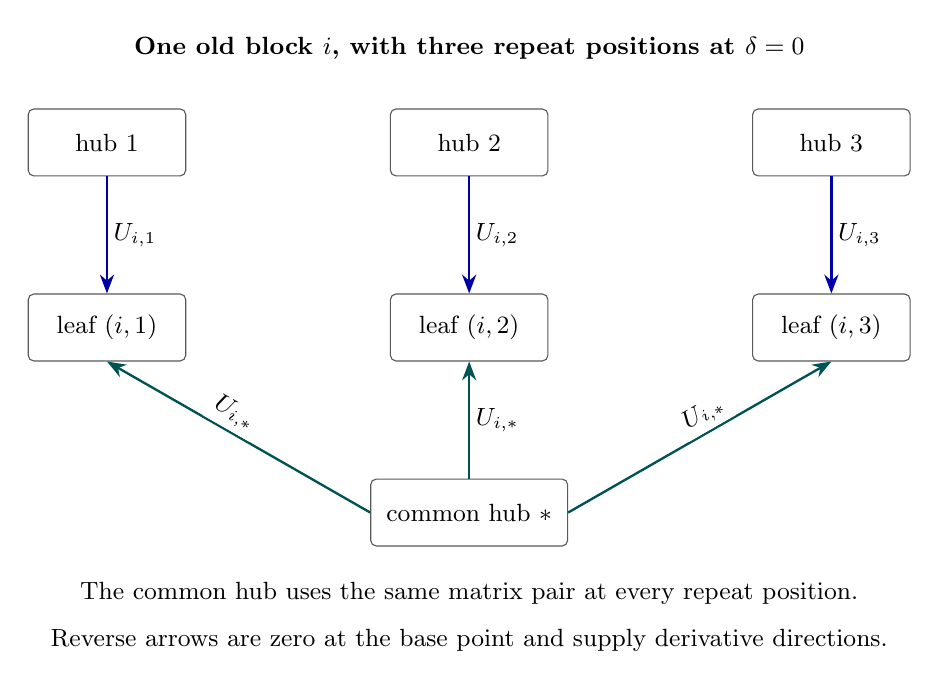
\begin{tikzpicture}[
  x=1cm,y=1cm,>=Stealth,
  every node/.style={font=\small},
  block/.style={rectangle,rounded corners=2pt,draw=black!65,fill=white,
    minimum width=20mm,minimum height=8.5mm,inner sep=4pt,align=center},
  forward/.style={draw=blue!65!black,line width=.85pt,->},
  common/.style={draw=teal!65!black,line width=.85pt,->},
  arrowlabel/.style={fill=white,inner sep=2pt}
]
  \node[font=\small\bfseries] at (6,5.9)
    {One old block $i$, with three repeat positions at $\delta=0$};
  \foreach \p/\xx in {1/1.4,2/6,3/10.6}{
    \node[block] (hub\p) at (\xx,4.7) {hub $\p$};
    \node[block] (leaf\p) at (\xx,2.35) {leaf $(i,\p)$};
    \draw[forward] (hub\p) --
      node[arrowlabel,right,pos=.5] {$U_{i,\p}$} (leaf\p);
  }
  \node[block,minimum width=25mm] (common) at (6,0) {common hub $*$};
  \draw[common] (common.west) --
    node[arrowlabel,above,sloped,pos=.55] {$U_{i,*}$} (leaf1.south);
  \draw[common] (common.north) --
    node[arrowlabel,right,pos=.5] {$U_{i,*}$} (leaf2.south);
  \draw[common] (common.east) --
    node[arrowlabel,above,sloped,pos=.55] {$U_{i,*}$} (leaf3.south);
  \node[align=center] at (6,-1.03)
    {The common hub uses the same matrix pair at every repeat position.};
  \node[align=center] at (6,-1.62)
    {Reverse arrows are zero at the base point and supply derivative directions.};
\end{tikzpicture}

\caption{The hub test at $\delta=0$, for one old block $i$ and $L=3$.
Hub $p$ sends a generic matrix pair only to position $p$; the common hub
sends the same pair to all positions. Every old block uses these same
$L+1$ hubs. At $\delta\ne0$ the leaf input may couple repeat positions.
The individual hubs eliminate off-diagonal dual entries, and the common
hub identifies the diagonal functionals.}
\label{fig:hub-test}
\end{figure}

Treat the entire deformed leaf array as one block and order it
before the hubs. Over the \(\delta\)-Laurent field this is a star
with maximal root count. Put
\[
 N=mL+L+1.
\]
Select the \(L\) branches over each old selected label and the
selected labels of all hubs, for a total of \(Na\) output rows.
The rank of their derivative matrix is at most
\(\rho_{bN}\leq Na-g\). This bound follows from the original
trace-minor identities, evaluated coefficientwise at the present
Taylor input; it does not require the specialized input to be
generic.

\newpage
\begin{lemma}[The limiting derivative columns]
\label{lem:limiting-columns}
The following derivative columns at the preceding star have finite
limits at \(\delta=0\).
\begin{enumerate}
\item A loop \(Y\otimes T\) inside old block \(i\) has limit
\[
 D_{i,h}(Y)\operatorname{tr}(\Pi_{i,h,j}T)
\]
on row \((i,h,j)\), and zero on all other rows. Hub loops give
their own loop responses.
\item For individual hub \(p\), a reverse arrow of value \(V\)
from repeat position \(r\) in old block \(i\) has limit
\begin{align*}
 &m_{i,h}(P_i,Q_p;U_{i,p},V)
      \operatorname{tr}(\Pi_{i,h,j}E_{pr})
       &&\text{on row }(i,h,j),\\
 &\mathbf 1_{p=r}\,
   m_{p,k}(Q_p,P_i;V,U_{i,p})
       &&\text{on hub row }(p,k),
\end{align*}
and zero elsewhere. Here \(E_{pr}\) is the repeat-factor matrix
unit with row \(p\) and column \(r\).
\item For the common hub, use arrow \(U_{i,*}\) and replace the
repeat-factor matrix by
\[
 \sum_{p=1}^L E_{pr}.
\]
The hub contribution is the single response
\(m_{*,k}(Q_*,P_i;V,U_{i,*})\).
\item The derivative along the whole input \(\delta\)-curve,
multiplied by \(\delta^{1-\ell}\), has limit
\(\ell\theta_{i,h,j}\) on leaf rows and zero on hub rows.
\end{enumerate}
The matrix consisting of a finite spanning collection of these
limiting columns has rank at most \(Na-g\).
\end{lemma}

\begin{proof}
Over the Laurent field, apply Lemma~\ref{lem:star-derivatives} with
the whole leaf array as one block. For loop derivatives, the
bounded leaf projection tends to
\(\pi_{i,h}\otimes\Pi_{i,h,j}\). Compression of the ordinary
first response gives \(D_{i,h}(Y)\) on the multiplicity space,
and taking trace divided by \(t\) gives the first formula.

For paired derivatives on a leaf, the Schur inverse is on the hub
at a root \(\lambda_{i,h,j}(\delta)\); that root stays away from
the hub spectrum at \(\delta=0\). For paired derivatives on a
hub, the inverse is on the leaf array at a hub root, which stays
away from every old leaf root. These inverses are regular at
\(\delta=0\). No inverse at the difference of two approaching
leaf roots occurs in this calculation.

At the reduction, the leaf input is diagonal between old blocks
and repeated inside each old block. A forward arrow at position
\(p\) followed by a reverse arrow from position \(r\) inserts
\(E_{pr}\) on the leaf repeat factor. At the hub end, the repeat
indices must match, giving \(\mathbf 1_{p=r}\). The ordinary
paired-response formula and trace divided by \(t\) now give the
second formula. Summing forward positions gives the common-hub
formula. The bounded projections and the distant-root inverses
justify all these limits coefficientwise.

The curve column lies in the span of input derivative columns over
the Laurent field by the chain rule. The expansion in
Lemma~\ref{lem:repeated-splitting} gives
\[
 \delta^{1-\ell}\frac{d}{d\delta}
       \lambda_{i,h,j}(\delta)
 =\ell\theta_{i,h,j}+O(\delta).
\]
Hub roots are constant on the curve. Thus this column also has a
finite limit. Choose bases for the finitely many loop and reverse
direction spaces and include the curve column. Every
\((Na-g+1)\)-minor of the resulting matrix vanishes over the
Laurent field; since its entries have finite limits, these minors
remain zero after specialization. This proves the last assertion.
\end{proof}

We now use the individual hubs to remove off-diagonal repeat-factor
weights and the common hub to make all diagonal weights agree.
The rank bound will then show that no element of \(\mathcal G\)
has been lost.

\begin{lemma}[The left nullspace]
\label{lem:hub-nullspace}
The left nullspace of the limiting matrix in
Lemma~\ref{lem:limiting-columns}, including its curve column,
has dimension \(g\). Its projection to the old blocks identifies
it with \(\mathcal G\): for each \(c\in\mathcal G\), its leaf
weights are \(c_{i,h}\) on every row \((i,h,j)\), independently
of \(j\), and its hub weights are the uniquely determined
compatible functionals. Consequently
\begin{equation}
 \sum_i\sum_{h\in I_i}c_{i,h}\operatorname{tr}(B_{i,h})=0
 \qquad(c\in\mathcal G).
 \label{eq:error-matrix-trace}
\end{equation}
\end{lemma}

\begin{proof}
Let \(\mu_{i,h,j}\) be leaf row weights in the left nullspace
and let \(\nu_p,\nu_*\) be the hub weights. Define
\[
 T_{i,h}=\sum_{j=1}^L\mu_{i,h,j}\Pi_{i,h,j}\in M_L(E).
\]
The loop columns imply
\[
 \sum_{h\in I_i}D_{i,h}(Y)
          \operatorname{tr}(T_{i,h}T)=0
 \qquad\text{for every }Y,T.
\]
Thus, for every matrix entry \((r,p)\), the coordinate vector
\( ((T_{i,h})_{rp})_{h\in I_i}\) defines a functional in
\(H_{P_i}^*\). The hub weights similarly belong to their own
loop annihilators.

Fix an individual hub \(p\) and a reverse position \(r\ne p\).
There is no hub response. Since
\[
 \operatorname{tr}(T_{i,h}E_{pr})=(T_{i,h})_{rp},
\]
the reverse columns say that the functional with these
\((r,p)\)-entries kills the leaf endpoint projection of the paired
map. That projection is onto \(H_{P_i}\), so all these entries
vanish. As \(p,r\) vary, every \(T_{i,h}\) is diagonal. When
\(r=p\), the corresponding diagonal-entry functional and the
hub functional \(\nu_p\) are exactly a pair in the relation of
Proposition~\ref{prop:compatible-relations}.

For the common hub, the leaf expression is
\[
 \operatorname{tr}\left(T_{i,h}\sum_pE_{pr}\right)
   =\sum_p(T_{i,h})_{rp}=(T_{i,h})_{rr}.
\]
For every \(r\), this diagonal-entry functional is therefore
paired with the same \(\nu_*\). Projection of the pair relation
onto the hub dual space is an isomorphism, so the diagonal-entry
functionals are independent of \(r\). Compatibility for the
collection of old blocks and hubs identifies them across all old
blocks. Hence
\[
 T_{i,h}=c_{i,h}I_L,
 \qquad c\in\mathcal G,
\]
and all hub weights are uniquely determined by \(c\). Since the
rank-one projections \(\Pi_{i,h,j}\) are mutually orthogonal
and sum to identity, this also gives
\(\mu_{i,h,j}=c_{i,h}\). The map from the left nullspace to
\(\mathcal G\) is consequently injective.

There are \(Na\) rows, and the limiting rank is at most \(Na-g\)
even after the curve column is included. The nullspace therefore
has dimension at least \(g\). Its injection into the
\(g\)-dimensional space \(\mathcal G\) is an isomorphism.
In particular every \(c\in\mathcal G\), not just a possible
subspace of relations, occurs. Pairing its null vector with the
curve column and cancelling the nonzero integer \(\ell\) yields
\[
 0=\sum_i\sum_{h\in I_i}\sum_{j=1}^L
       c_{i,h}\theta_{i,h,j}
  =\sum_i\sum_{h\in I_i}c_{i,h}\operatorname{tr}(B_{i,h}).
\]
If \(g=0\), the same proof gives zero nullspace and the assertion
about \(c\) is vacuous. If \(L=1\), the off-diagonal step has
no entries to remove; the common-hub step still gives precisely
the stated conclusion.
\end{proof}

\begin{proof}[Proof of Theorem~\ref{thm:cyclic-compatibility}]
Apply Lemma~\ref{lem:hub-nullspace} to arbitrary \(S_1,S_2\)
and to the auxiliary loops chosen in
Lemma~\ref{lem:repeated-splitting}. The added-loop contribution
to \eqref{eq:error-matrix-trace} is zero. Indeed, write
\(Y_i=\sum_\alpha Y_{i,\alpha}\otimes T_{i,\alpha}\). Then
\[
 \sum_{h\in I_i}c_{i,h}\operatorname{tr}(D_{i,h}(Y_i))
 =\sum_\alpha\operatorname{tr}(T_{i,\alpha})
      \sum_{h\in I_i}c_{i,h}D_{i,h}(Y_{i,\alpha})=0,
\]
because \(c_i\) annihilates the loop image. We conclude that,
for arbitrary matrix substitutions,
\begin{equation}
 \sum_{|\omega|=\ell}
 \left(\sum_i\sum_{h\in I_i}c_{i,h}e_{i,h,\omega}\right)
 \operatorname{tr}(S^\omega)=0.
 \label{eq:all-matrix-trace-tests}
\end{equation}
Auxiliary field extensions impose no restriction: this equality
has its coefficients in the original field, and extension is
injective.

We use a matrix-cycle test of the kind appearing in the constructive
trace argument of \cite[Proposition~4.1]{KlepSpenko2014}, recording the
rotational multiplicity explicitly. Fix a word
\(\omega_0=c_0c_1\cdots c_{\ell-1}\), with letters
\(c_j\in\{1,2\}\), and take \(L=\ell\). On vertices indexed
modulo \(\ell\), set
\[
 S_c=\sum_{j:\,c_j=c}E_{j,j+1}\qquad(c=1,2).
\]
For a word \(\omega\) of length \(\ell\), its matrix trace
counts the starting vertices at which one reads \(\omega\)
around this directed cycle. It is zero unless \(\omega\) lies
in the cyclic orbit \(\mathcal O\) of \(\omega_0\); for every
distinct word in that orbit its value is the same positive integer
\[
 \frac{\ell}{|\mathcal O|}.
\]
This is the rotational stabilizer size and includes periodic and
constant-letter words. Substitution into
\eqref{eq:all-matrix-trace-tests}, followed by cancellation of that
integer in characteristic zero, gives
\eqref{eq:cyclic-error-relation}.
\end{proof}

The leading errors now satisfy every cyclic relation imposed by
\(\mathcal G\). The colored correction graph will make these
exactly the annihilators of its order-by-order correction map.

\section{Solving the free-series equations}
\label{sec:free-correction}

We now use the response and cyclic-sum results to keep the output of a
substitution conjugate to its constant term.  The input retains two prescribed
linear coefficients.  This is the point at which free words, rather than
commuting parameters, enter the construction essentially.

Work over a common split scalar field $E$ in which the preceding evaluations
and spectral projections are defined.  All series substitutions below have
small constant terms and are interpreted by the coefficientwise valuation
convergence established earlier.  In particular, the letters of a free series
commute with its matrix coefficients; the letters do not commute with each
other.

Put $m=11$ and index the blocks by $i\in\mathbb Z/m\mathbb Z$.
Let $P_i$ be jointly independent small generic pairs of $b\times b$
matrices.  Set $R=\operatorname{diag}(P_i)$, a pair of $mb\times mb$
matrices.  The old coefficient algebra acts on a separate factor of dimension
$d$.  Write $\lambda_{i,h}$ and $\pi_{i,h}$ for the distinct eigenvalues
and spectral projections of $w(P_i)$.  Eigenvalues belonging to different
blocks are distinct.  For a substitution $Z$ with constant term $R$, let
$S_{i,h}(Z)$ denote the fixed-root Schur expression at $\lambda_{i,h}$,
using the constant projection $\pi_{i,h}$ in the $i$-th block.

We recall precisely the response information needed here.  In each block
choose one eigenvalue label from every part of the active partition, giving
$a$ selected labels.  The selected loop-response map is
\[
 D_i:M_b(E)^2\longrightarrow E^a.
\]
Put $L_i=\operatorname{im}D_i$ and $H_i=E^a/L_i$.
Proposition~\ref{prop:compatible-relations} supplies a vector space
$G=\mathcal G$ of dimension $g$ and coordinate isomorphisms
\[
 p_i:G\longrightarrow H_i^*.
\]
For a generic fixed input arrow $U$ on $i\leftarrow j$, varying its
opposite arrow $V$ gives two selected responses
\[
 m_i(U,V)\in E^a,
 \qquad m_j(V,U)\in E^a.
\]
The annihilator of these paired responses in $H_i^*\oplus H_j^*$ is
exactly
\begin{equation}
 \{(p_i(c),p_j(c)):c\in G\}.
 \label{eq:correction-paired-annihilator}
\end{equation}
The identifications $p_i$ are compatible for the whole collection of blocks
and for all the generic arrows used below.

The transfer result supplies the following additional facts.  If all Schur
expressions vanish in degrees less than $\ell$, their degree-$\ell$
coefficients are scalar on the projected eigenspaces.  The resulting tuples
belong to their active spaces and are determined by their selected entries.
Denote the selected error for a word $\omega$ of length $\ell$ in block
$i$ by $e_{i,\omega}\in E^a$.  The cyclic-sum result says that, for every
orbit $\mathcal O$ of words under cyclic rotation,
\begin{equation}
 \sum_{\omega\in\mathcal O}\sum_i
 p_i(c)\bigl(e_{i,\omega}+L_i\bigr)=0
 \qquad(c\in G).
 \label{eq:correction-cyclic-input}
\end{equation}
These statements hold for every partial substitution under consideration,
including after an extension of its scalar field.  The preceding results
therefore supply all the hypotheses used in the next construction.

\begin{proposition}
\label{prop:eleven-block-correction}
Prescribe generic input-arrow pairs on the edges
\[
 \begin{array}{c|c}
 \text{letter}&\text{offsets }i-j\text{ of edges }i\leftarrow j\\ \hline
 s_1&1,2\\
 s_2&3,4.
 \end{array}
\]
Under the response and cyclic-sum hypotheses above, there is a pair
$Z(s_1,s_2)\in M_{mb}(E)\langle\!\langle s_1,s_2\rangle\!\rangle^2$
with constant term $R$ and exactly these prescribed linear coefficients,
for which
\[
 S_{i,h}(Z)=0\qquad\text{for every }i,h.
\]
It can be constructed by finite linear systems.  At step $\ell\ge3$ the
new unknowns are coefficients of degree $\ell-1$ on the reverse edges
and coefficients of degree $\ell$ on the diagonal blocks.
\end{proposition}

\begin{proof}
None of the four forward offsets is zero.  The sum of two forward offsets
lies between $2$ and $8$, and is therefore nonzero modulo $11$.
Thus a path of one or two forward steps cannot return to its initial block.
Constant input steps preserve each block.  The path expansions for the
output and for its Schur expressions consequently show that the prescribed
constant and linear terms, with zero higher coefficients, solve all the
Schur equations through degree two.

Suppose a partial substitution solves them in degrees less than
$\ell\ge3$.  Add a correction $V B$ on a reverse edge $j\leftarrow i$,
where $B$ is a word of length $\ell-1$, and add arbitrary degree-$\ell$
loop corrections.  At the block-diagonal constant term, an off-diagonal
input variation gives an output variation in the same off-diagonal block.
Its compression on any fixed root block is zero.  Thus the reverse
correction changes no Schur equation through degree $\ell-1$.

Its contribution in degree $\ell$ must pair it with a single prescribed
linear arrow.  There is a unique forward edge that returns along this
reverse edge: the reverse offsets $10,9,8,7$ correspond respectively to
$1,2,3,4$.  If that edge has coefficient $U$ and color $s_c$, the
contributions are
\begin{equation}
 \begin{array}{c|c|c}
 \text{block}&\text{word}&\text{selected response}\\ \hline
 i&s_cB&m_i(U,V)\\
 j&Bs_c&m_j(V,U).
 \end{array}
 \label{eq:correction-leading-pair}
\end{equation}
This is exactly the two-arrow Schur calculation defining the paired
responses.  A previously present coefficient of degree at least two
cannot interact with the new degree-$\ell-1$ coefficient in degree
$\ell$.  Two new corrections have total degree at least
$2(\ell-1)>\ell$.  The degree-$\ell$ variation is therefore linear.
Loop corrections give $D_i$ independently at every vertex and every
word of length $\ell$.

We compute the annihilator of this finite correction map.  Let
$f_{i,\omega}\in(E^a)^*$ be a collection of functionals annihilating its
image.  The loop columns first imply that $f_{i,\omega}$ annihilates
$L_i$.  Write its induced functional on $H_i$ uniquely as
\[
 f_{i,\omega}=p_i(c_{i,\omega}),\qquad c_{i,\omega}\in G.
\]
Here and below we use the same notation for the induced functional and
its pullback to $E^a$.  By
\eqref{eq:correction-paired-annihilator} and
\eqref{eq:correction-leading-pair}, annihilation of the reverse columns
is equivalent to
\begin{equation}
 c_{i,s_cB}=c_{j,Bs_c}
 \quad\text{on every edge }i\leftarrow j\text{ of color }c.
 \label{eq:correction-edge-equality}
\end{equation}
The two offsets of either color are consecutive integers, say $a,a+1$.
Applying \eqref{eq:correction-edge-equality} to both edges out of $j$
gives
\[
 c_{j+a,s_cB}=c_{j+a+1,s_cB}.
\]
As $j$ ranges over $\mathbb Z/11\mathbb Z$, this makes the value
independent of the vertex.  Equation~\eqref{eq:correction-edge-equality}
then identifies its value with that on the rotated word $Bs_c$.
Iterating rotations shows that the annihilator consists exactly of one
element of $G$ per cyclic orbit of words.  The converse follows from
the same paired-annihilator identity.

Equation~\eqref{eq:correction-cyclic-input} says that every such
annihilator kills the degree-$\ell$ error.  Finite-dimensional linear
duality therefore puts the negative error in the image of the correction
map.  Choose a correction solving all selected equations.  Lower degrees
remain solved, so transfer and the active partition imply that every
nonselected equation vanishes in degree $\ell$ as well.

Continue inductively.  A coefficient of degree $n$ can change only at
steps $n$ and $n+1$, so the resulting free series is well-defined.
Every fixed Schur coefficient is eventually zero and remains zero.
The construction also covers $g=0$, when the annihilator is zero.
For a periodic word the orbit consists of its distinct rotations; no
multiplicity is inserted into the annihilator calculation or into
\eqref{eq:correction-cyclic-input}.
\end{proof}

\begin{figure}[tbp]
\centering
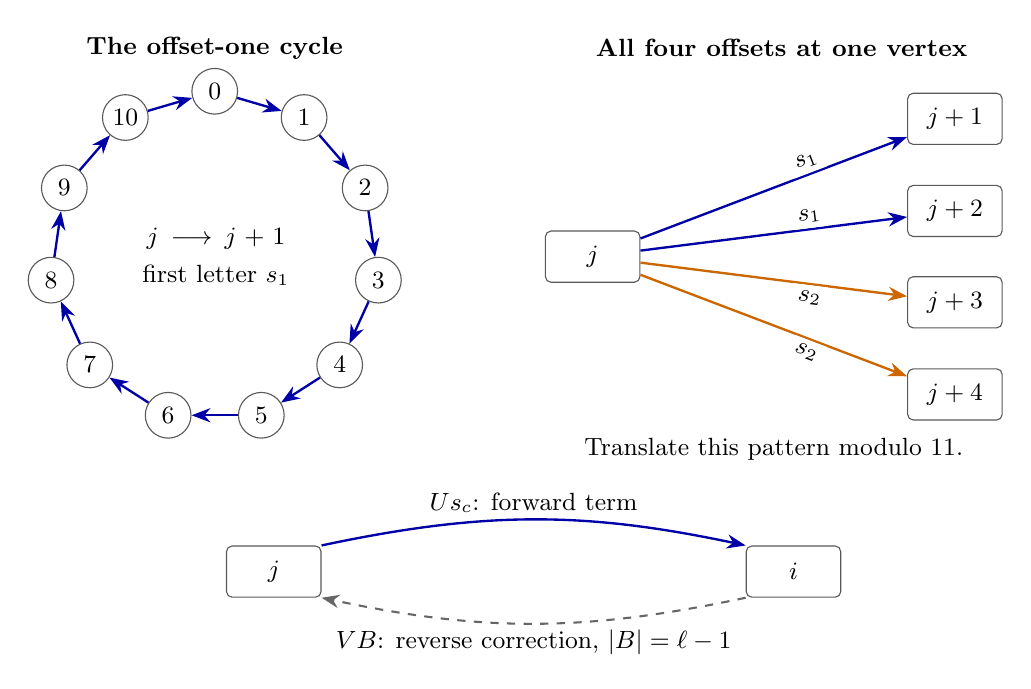
\begin{tikzpicture}[
  x=1cm,y=1cm,>=Stealth,
  every node/.style={font=\small},
  vertex/.style={circle,draw=black!65,fill=white,minimum size=5.8mm,inner sep=1.5pt},
  block/.style={rectangle,rounded corners=2pt,draw=black!65,fill=white,
    minimum width=12mm,minimum height=6.5mm,inner sep=3pt},
  first/.style={draw=blue!65!black,line width=.85pt,->},
  second/.style={draw=orange!80!black,line width=.85pt,->},
  correction/.style={draw=black!60,line width=.75pt,dashed,->},
  arrowlabel/.style={fill=white,inner sep=2pt}
]
  \node[font=\small\bfseries] at (2.45,5.55) {The offset-one cycle};
  \foreach \j in {0,...,10}{
    \node[vertex] (v\j) at ({2.45+2.1*cos(90-360*\j/11)},
                             {2.9+2.1*sin(90-360*\j/11)}) {$\j$};
  }
  \foreach \j in {0,...,10}{
    \pgfmathtruncatemacro{\next}{mod(\j+1,11)}
    \draw[first] (v\j) -- (v\next);
  }
  \node[align=center,text width=27mm] at (2.45,2.9)
    {$j\longrightarrow j+1$\\[3pt]first letter $s_1$};
  \node[font=\small\bfseries] at (9.65,5.55) {All four offsets at one vertex};
  \node[block] (j) at (7.25,2.9) {$j$};
  \node[block] (j1) at (11.85,4.65) {$j+1$};
  \node[block] (j2) at (11.85,3.48) {$j+2$};
  \node[block] (j3) at (11.85,2.32) {$j+3$};
  \node[block] (j4) at (11.85,1.15) {$j+4$};
  \draw[first] (j) -- node[arrowlabel,pos=.64,above,sloped] {$s_1$} (j1);
  \draw[first] (j) -- node[arrowlabel,pos=.64,above,sloped] {$s_1$} (j2);
  \draw[second] (j) -- node[arrowlabel,pos=.64,below,sloped] {$s_2$} (j3);
  \draw[second] (j) -- node[arrowlabel,pos=.64,below,sloped] {$s_2$} (j4);
  \node[align=center] at (9.55,.45) {Translate this pattern modulo $11$.};
  \node[block] (pairj) at (3.2,-1.1) {$j$};
  \node[block] (pairi) at (9.8,-1.1) {$i$};
  \draw[first] (pairj.north east) to[bend left=12]
    node[arrowlabel,above] {$U s_c$: forward term} (pairi.north west);
  \draw[correction] (pairi.south west) to[bend left=12]
    node[arrowlabel,below] {$V B$: reverse correction, $|B|=\ell-1$} (pairj.south east);
\end{tikzpicture}

\caption{The eleven-block input pattern. Indices lie in $\mathbb Z/11\mathbb Z$.
The left panel shows the offset-one cycle; the right panel specifies all
four forward offsets, translated at every vertex. Each forward arrow carries a
generic pair of input matrices. At order $\ell\ge3$, a reverse correction
has degree $\ell-1$; degree-$\ell$ loop corrections are not drawn.}
\label{fig:eleven-blocks}
\end{figure}

Figure~\ref{fig:eleven-blocks} separates the generating cycle from the
full local arrow pattern. The role of the four offsets is now explicit.  Avoiding returns of length
one or two starts the induction without changing the linear data.
Consecutive offsets within each color make its only obstructions
independent of the vertex.  The remaining obstructions are exactly the
cyclic sums already proved to vanish.

\subsection{Fixed roots and Schur complements}

The following elementary fact identifies the spectral equations with a
single polynomial identity. Its coefficient ring need not be commutative.
Let $E$ be a field, let $\mathfrak a=(s_1,s_2)$ be the augmentation ideal
of the free algebra $E\langle s_1,s_2\rangle$, and put
\[
  T_N=E\langle s_1,s_2\rangle/\mathfrak a^{N+1}
  \qquad (N\geq 0).
\]
Elements of $E$ are central in $T_N$. Reduction modulo $\mathfrak a$
is called the constant term.

\begin{lemma}\label{lem:schur-polynomial}
Let $W\in M_d(T_N)$ have constant term
\[
  W_0=\sum_{h=1}^{e}\lambda_h\pi_h,
  \qquad
  \pi_h\pi_j=\delta_{hj}\pi_h,
  \qquad
  \sum_{h=1}^{e}\pi_h=I_d,
\]
where the $\lambda_h\in E$ are distinct and the $\pi_h\in M_d(E)$
are nonzero projections. Set
\[
  q(t)=\prod_{h=1}^{e}(t-\lambda_h),
  \qquad \bar\pi_h=I_d-\pi_h.
\]
On the complementary summand $\bar\pi_h T_N^d$, the operator
\[
  C_h=\bar\pi_h(W-\lambda_h I_d)\bar\pi_h
\]
is invertible. Define the Schur expression on $\pi_h T_N^d$ by
\[
  S_h=\pi_h(W-\lambda_h I_d)\pi_h
      -\pi_hW\bar\pi_h C_h^{-1}\bar\pi_hW\pi_h.
\]
Then $q(W)=0$ if and only if $S_h=0$ for every $h$.
\end{lemma}

\begin{proof}
The constant term of $C_h$ is
$\sum_{j\ne h}(\lambda_j-\lambda_h)\pi_j$, which is invertible on
$\bar\pi_h E^d$. A matrix over $T_N$ with invertible constant term is
invertible: after factoring out its constant term, the inverse is a
finite geometric series in a matrix with entries in $\mathfrak a$.
This proves the assertion about $C_h$. All modules below are right
$T_N$-modules, with matrices acting on column vectors from the left.

Suppose first that every $S_h$ vanishes. Define
$K_h:\pi_hT_N^d\longrightarrow T_N^d$ by
\[
  K_hu=u-C_h^{-1}\bar\pi_hW\pi_hu,
\]
where the second term lies in the complementary summand. Then
$\pi_hK_hu=u$, and direct block multiplication gives
\[
  (W-\lambda_h I_d)K_hu=S_hu=0.
\]
The map $K=\sum_hK_h\pi_h$ has constant term $I_d$, so it is
invertible. The displayed kernel equations imply
$WK=KW_0$. Consequently
\[
  q(W)=Kq(W_0)K^{-1}=0.
\]

Conversely, suppose $q(W)=0$. Define
\[
  P_h=\prod_{j\ne h}
       \frac{W-\lambda_j I_d}{\lambda_h-\lambda_j}.
\]
These products are unambiguous because their factors are polynomials
in the same matrix with central scalar coefficients. Polynomial
interpolation modulo $q$ shows that the $P_h$ are spectral
idempotents; in particular,
\[
  (W-\lambda_h I_d)P_h=0,
  \qquad P_h\equiv\pi_h\pmod{\mathfrak a}.
\]
Let $\iota_h:\pi_hT_N^d\longrightarrow T_N^d$ be inclusion. The
endomorphism $A_h=\pi_hP_h\iota_h$ of $\pi_hT_N^d$ has constant
term the identity, and is therefore invertible. Thus
\[
  \widetilde K_h=P_h\iota_hA_h^{-1}
\]
satisfies
$\pi_h\widetilde K_h=\operatorname{id}_{\pi_hT_N^d}$ and
$(W-\lambda_h I_d)\widetilde K_h=0$. The complementary component
of the latter equation determines its remaining component uniquely:
\[
  \bar\pi_h\widetilde K_h
    =-C_h^{-1}\bar\pi_hW\pi_h.
\]
Its $\pi_h$ component now gives $S_h=0$.
\end{proof}

For a matrix over $E\langle\!\langle s_1,s_2\rangle\!\rangle$,
apply Lemma~\ref{lem:schur-polynomial} after reduction to $T_N$.
It follows that the fixed-root Schur equations hold through degree
$N$ exactly when the identity $q(W)=0$ holds through degree $N$.
In particular, this equivalence applies at every finite stage of a
formal correction, with the same polynomial $q$ throughout.

\section{Realization in a central division algebra}
\label{sec:division-realization}

The preceding construction solved equations in split matrices.  We now
place its constant blocks and prescribed arrows in one central division
algebra.  Each subsequent correction is the solution of a finite linear
system over its center.  This permits descent without any assertion that
solutions of nonlinear equations descend.

Throughout this section $k$ has characteristic zero and contains all roots
of unity, and $A$ is a central division algebra of degree $d$ over $k$.
The integer $b$ is the block size chosen earlier in the spectral case.
In the case where $q_0(w)=0$ already holds as a free-series identity, any
positive integer $b$ may be used.  Put $m=11$.

\subsection{The two division-algebra factors}

Choose independent central indeterminates $\alpha,\beta$ and put
$k_0=k(\alpha,\beta)$.  Let $B_b$ be the symbol algebra over $k_0$
generated by $u,v$ with
\[
 u^b=\alpha,\qquad v^b=\beta,\qquad vu=\zeta_buv,
\]
where $\zeta_b$ is a primitive $b$-th root of unity.  For $b=1$ this
means $B_1=k_0$.  By the construction in Section~\ref{subsec:generic-division}, $B_b$
is central simple of degree $b$.  Lemma~\ref{lem:symbol-division}
shows that $A\otimes_k B_b$ is division and remains division under
pure rational and central Laurent scalar extensions.  We will use
these facts twice in adjoining the cyclic block factor.

Fix a $k_0$-basis $(e_a)_{a=1}^{b^2}$ of $B_b$.  Over $k_0$ introduce
the following jointly independent variables:
\[
 x_{c,a,j},\qquad y_{r,c,a,j},
 \qquad
 \begin{matrix}
 c\in\{1,2\},\quad 1\le a\le b^2,\\
 j\in\mathbb Z/m\mathbb Z,\quad r\in\{1,2,3,4\}.
 \end{matrix}
\]
Let $L_0$ be their rational function field and let $\sigma$ increase
the index $j$ by one, fixing $k_0$.  This automorphism has order exactly
$m$.  Put $H_0=L_0^{\langle\sigma\rangle}$.  Artin's fixed-field theorem
for a finite group of automorphisms gives a cyclic Galois extension
$L_0/H_0$ of degree $m$; see \cite[Corollary~3.11, p.~38]{MilneFT2022}.

Choose a further independent central indeterminate $a_*$ and form the
cyclic algebra $C$ over $F_0=H_0(a_*)$ with coefficient field
$L_0(a_*)$ and generator $\tau$, subject to
\begin{equation}
 \tau^m=a_*,\qquad \tau c\tau^{-1}=\sigma(c)
 \quad(c\in L_0).
 \label{eq:cyclic-realization-relations}
\end{equation}
It has vector-space decomposition
$C=\bigoplus_{r=0}^{m-1}L_0(a_*)\tau^r$.
After extending scalars to a field containing $L_0(a_*)$, represent
$c\in L_0$ by the diagonal with entries $\sigma^{-i}(c)$ and
$\tau$ by the cyclic forward shift, whose wrap entry is $a_*$.
These matrices satisfy \eqref{eq:cyclic-realization-relations} and
span all matrix units.  This gives the usual splitting of $C$ and
shows that it is central simple of degree $m$; see
\cite[Construction~2.5.1 and Proposition~2.5.2]{GilleSzamuely2006}.
Our conjugation convention uses the inverse of their Galois generator.

Define
\[
 \widetilde B_0=(B_b\otimes_{k_0}F_0)\otimes_{F_0}C,
 \qquad D_0=A\otimes_k\widetilde B_0.
\]
Then $D_0$ is central simple of degree $dbm$ over $F_0$ by the tensor-product and scalar-extension properties of
central simple algebras
\cite[Chapter~IV, Corollary~2.8 and Proposition~2.15]{MilneCFT}.
It is also division. Indeed
\[
 D_L=(A\otimes_k B_b)\otimes_{k_0}L_0
\]
is division by the rational-extension argument.  Extend $\sigma$ to
$D_L$ by fixing the old algebra factors.  The skew Laurent division
ring $D_L((t;\sigma))$ receives a unital homomorphism from $D_0$
by $\tau\mapsto t$ and $a_*\mapsto t^m$.  The central element
$t^m$ is transcendental over $H_0$.  Simplicity again makes this map
injective, and finite dimension makes $D_0$ division.

Finally put
\[
 F=F_0((\varepsilon)),\qquad
 \widetilde B=\widetilde B_0\otimes_{F_0}F,\qquad
 D=D_0\otimes_{F_0}F.
\]
The central Laurent argument shows that $D$ is a central division
algebra over $F$ of degree $dbm$.  Input coefficients will lie in
$\widetilde B$, so that they commute with the old factor $A$.

\subsection{One realization of all generic data}

For $r\in\mathbb Z/m\mathbb Z$, let
\[
 \mathcal V_r=
 \bigl(B_b\otimes_{k_0}L_0\bigr)\tau^r
 \otimes_{H_0}F
 \ \subseteq\ \widetilde B.
\]
This notation uses the evident coefficient embedding and scalar
extension; equivalently it is the $F$-span of that graded summand in
$\widetilde B_0$.  Upon splitting, $\mathcal V_r$ consists exactly
of all $b\times b$ entries at offset $r$ in the $m$-block matrix.
In fact $L_0\otimes_{H_0}E\simeq E^m$ over a splitting field $E$,
and $B_b$ becomes $M_b(E)$.  Multiplication by $\tau^r$ moves these
independent diagonal entries to offset $r$, with nonzero wrap factors.
In particular $\mathcal V_0$ gives all diagonal blocks, and
$\mathcal V_{-r}$ gives all reverse entries for offset $r$.

Define the two constant inputs and four arrow pairs by
\[
 P_c^0=\varepsilon\sum_a x_{c,a,0}e_a,
 \qquad
 U_{r,c}=\left(\sum_a y_{r,c,a,0}e_a\right)\tau^r
 \quad(c=1,2).
\]
The prescribed initial substitution is the pair
\begin{equation}
 Z_c^{\mathrm{init}}(s_1,s_2)
 =P_c^0+(U_{1,c}+U_{2,c})s_1
             +(U_{3,c}+U_{4,c})s_2.
 \label{eq:division-initial-input}
\end{equation}
After splitting, the diagonal blocks of $(P_1^0,P_2^0)$ are exactly
the required independent small generic pairs.  The two input-component
entries at every forward edge are independent generic entries, jointly
with all the diagonal data.

Here independence is over the old split coefficient field, which is the
field used in the generic rank tests.  To check it, first split $A$ and
$B_b$ using constants independent of the variables $x,y$.  The $m$
conjugates of each coefficient use the disjoint sets of variables with
different index $j$.  The split symbol basis is a matrix basis.
Permuting those variables, changing that basis, and multiplying entries
by powers of $a_*$ preserve their algebraic independence.  This verifies
all generic determinant conditions simultaneously.  No independence
over the larger invariant field $H_0$ is asserted or needed.

We may perform the spectral calculations after extending $F$ to a
split Laurent field and then to the finite extensions needed for
eigenvalues.  Its constant coefficient field contains the old algebraic
closure and the rational variables just chosen.  The matrix constant
terms remain $\varepsilon$-small.  Arrow coefficients need not be
small, since they occur only with positive free-word degree.

\subsection{Linear descent of the correction}

Assume first that $q_0(w)\ne0$.  Let $W_0=w(P_1^0,P_2^0)\in D$
and choose its monic minimal polynomial
\begin{equation}
 q(t)\in F[t].
 \label{eq:fixed-central-polynomial}
\end{equation}
We keep this polynomial fixed throughout the correction.  It is
irreducible, because $F[W_0]$ is a finite-dimensional commutative
domain, and separable because the characteristic is zero.  In a
splitting field its roots are exactly the distinct eigenvalues of the
constant output.  For completeness, left multiplication by $W_0$ on
$D$ has characteristic polynomial a power of $q$, since $D$ is a
vector space over $F[W_0]$.  After splitting, that left multiplication
is a direct sum of copies of the action of the split matrix $W_0$.
Every root of $q$ therefore occurs in that matrix, and no other
eigenvalue occurs.  Separability makes its action semisimple.

We solve $q(w(Z))=0$ in free series over $D$.  Initially take
\eqref{eq:division-initial-input}.  Its split Schur equations vanish
through degree two, so Lemma~\ref{lem:schur-polynomial} gives the same
assertion for the polynomial relation.  Suppose inductively that a
partial substitution solves this relation through degree $\ell-1$,
where $\ell\ge3$.  Allow a new coefficient in
$\mathcal V_{-r}^2$ at every word of length $\ell-1$, for
$r=1,2,3,4$, and a new coefficient in $\mathcal V_0^2$ at every word
of length $\ell$.  These are finite-dimensional $F$-spaces.

Impose every coefficient equation of
\begin{equation}
 q(w(Z))=0\pmod{(s_1,s_2)^{\ell+1}}.
 \label{eq:finite-central-correction}
\end{equation}
This is a finite affine linear system over $F$ in the allowed new
coordinates.  Indeed two new insertions have degree at least
$2(\ell-1)>\ell$.  At any fixed free-word degree, only boundedly
many positive-degree insertions occur in the evaluation of the old
series; the remaining insertions are from the $\varepsilon$-small
constant input.  The finitely many previously fixed coefficients have
a finite lower valuation bound.  Thus the sums defining each
coefficient of \eqref{eq:finite-central-correction}, and its linear
part in the new coordinates, converge in $D$ and are defined over $F$.
Choosing an $F$-basis of $D$ turns them into finitely many ordinary
scalar linear equations.

After scalar extension, each permitted input space becomes exactly
the collection of reverse edges or loops used in
Proposition~\ref{prop:eleven-block-correction}.  The current partial
substitution is a valid partial split solution by
Lemma~\ref{lem:schur-polynomial}.  The proposition supplies a split
correction, and that lemma converts its Schur vanishings back to all
the equations in \eqref{eq:finite-central-correction}.  In particular
the new degree-$\ell-1$ reverse coefficients preserve the already
solved equations: their diagonal Schur variation at that degree is
zero.  We have therefore solved the whole finite linear system after
a field extension.  A matrix and its augmented matrix have the same
ranks before and after extension, so the system already has a solution
over $F$.

Choose such a solution at every step.  The coefficient stabilization
in Proposition~\ref{prop:eleven-block-correction} produces
\[
 Z\in\widetilde B\langle\!\langle s_1,s_2\rangle\!\rangle^2,
 \qquad q(w(Z))=0,
\]
with the prescribed constant and linear terms.  Only finite linear
systems have been descended.  Neither the roots of $q$ nor the split
correction coefficients need belong to $F$.

Since the input coefficients commute with $A$, evaluation at $Z$
defines a substitution homomorphism
\[
 A\langle\!\langle z_1,z_2\rangle\!\rangle
 \longrightarrow D\langle\!\langle s_1,s_2\rangle\!\rangle.
\]
It is well-defined by the same coefficientwise valuation bound: at
fixed output degree, only boundedly many nonconstant input factors
occur.  The bound also justifies multiplication and regrouping of the
convergent coefficient sums.  Hence every old polynomial identity on
the tuple and the chosen series is preserved by this substitution.

If $q_0(w)=0$ already holds, use the very same division algebra and
the initial substitution \eqref{eq:division-initial-input}, with any
$b\ge1$.  No spectral correction is required; the old relation
$q_0(w)$ remains zero under the substitution homomorphism.  Both cases
produce a central division algebra of degree $11bd>d$, with identical
generic forms for the constant and the two linear input coefficients.
The next step restores generation and two transverse directions using
these coefficients.  That step is needed in the unconstrained case
as well as in the spectral case.

\section{Restoring generation and two transverse directions}
\label{sec:generation}

The preceding construction gives a substitution $Z(s_1,s_2)$ inside
the centralizer of $A$ in a larger central division algebra.  It
preserves the old polynomial identities and algebraizes the chosen
series.  To complete Theorem~\ref{thm:lifting}, we must
make the new constant tuple generate the larger algebra and retain
two independent directions modulo inner derivations. We first use the
original transverse directions to prove generation of the generic
diagonal product and to control the arrows between its blocks.
Translating the first free letter by a new central parameter then joins
the blocks into a full matrix algebra. A single rank calculation shows
that both directions remain independent modulo inner derivations.

Throughout this section, brackets with a tuple are taken componentwise.
Thus, for $C=(C_1,\ldots,C_u)$ in an algebra $B$, write
\[
 J(C)=\{([T,C_1],\ldots,[T,C_u]):T\in B\}.
\]
Polynomial relations on $X_0$ detect the two input directions to first
order.

\begin{lemma}[Derivatives of relations]
\label{lem:derivatives-of-relations}
Let $A$ be a finite-dimensional central simple algebra over a field
$k$ of characteristic zero.  Let
$X\in A\langle\!\langle z_1,z_2\rangle\!\rangle^u$ have constant
tuple $X_0$ generating $A$, and suppose its two linear coefficients
$X_1,X_2$ are independent modulo $J(X_0)$.  Define
\[
 \theta:k\langle x_1,\ldots,x_u\rangle\longrightarrow A,
 \qquad \theta(f)=f(X_0),\qquad I=\ker\theta.
\]
Then the map taking $f\in I$ to the coefficients of $z_1,z_2$ in
$f(X)$ is onto $A^2$.
\end{lemma}

\begin{proof}
Denote these two coefficient maps by $\delta_1,\delta_2$.  Each
satisfies
\[
 \delta_j(fg)=\theta(f)\delta_j(g)+\delta_j(f)\theta(g).
\]
Since $\theta$ is onto and $I$ is a two-sided ideal, the image
$M=(\delta_1,\delta_2)(I)$ is an $A$-bimodule in $A^2$.

Left and right multiplication generate $\operatorname{End}_k(A)$;
see \cite[Chapter~IV, Corollary~2.9]{MilneCFT}.
Indeed, after splitting $A$, multiplication by matrix units on the
left and right gives every matrix unit on the vector space $A$;
the resulting isomorphism
$A\otimes_k A^{\mathrm{op}}\simeq\operatorname{End}_k(A)$ descends
by finite-dimensional linear algebra.  Applying these endomorphism
matrix units to $M\subseteq A\otimes_k k^2$ shows that
$M=A\otimes_k V$ for a subspace $V\subseteq k^2$.
If $V\ne k^2$, some nonzero $(a,b)\in k^2$ annihilates $V$.
The map $a\delta_1+b\delta_2$ then vanishes on $I$ and descends to
a derivation of $A$.

Every $k$-linear derivation of $A$ is inner
\cite[Theorem~8]{Jacobson1937Derivations}. For completeness, after
splitting $A=M_d(E)$, a derivation $\partial$ is implemented by
\[
 T=\sum_i\partial(E_{i1})E_{1i}.
\]
Differentiating $E_{kl}E_{i1}=\delta_{li}E_{k1}$, multiplying by
$E_{1i}$, and summing gives $\partial(E_{kl})=[T,E_{kl}]$.
The equations for an implementing element on a fixed $k$-basis of
$A$ form a linear system over $k$.  Solvability after scalar
extension implies solvability over $k$.
It follows that $aX_1+bX_2\in J(X_0)$, a contradiction.
\end{proof}

In particular, there are $f_1,f_2\in I$ whose derivative pairs are
$(1,0)$ and $(0,1)$.  These relations recover the two generic input
matrices from small evaluations of the tuple.

\begin{lemma}[Generic blocks]
\label{lem:generic-generating-blocks}
Under the hypotheses of Lemma~\ref{lem:derivatives-of-relations},
write $d=\deg A$ and split $A$ into $d\times d$ matrices.  Fix a
positive integer $b$ and finitely many independent small generic input pairs
\[
 P_i=\varepsilon P_i^{\circ},\qquad 1\le i\le r,
\]
of $b\times b$ matrices, with jointly independent entries in the
$P_i^{\circ}$.  Work over a common splitting Laurent field.
Then each tuple $C_i=X(P_i)$ generates $M_{db}$, and the diagonal
tuple $C=\operatorname{diag}(C_i)$ generates the full product of
these matrix algebras.

For distinct $i,j$, the output derivative of a generic input arrow
$U=(U_1,U_2)$ from block $j$ to block $i$ is nonzero modulo
\[
 \{C_iT-TC_j:T\in M_{db}\}.
\]
More precisely, the image of the arrow derivatives in this quotient
has dimension at least $b^2$.
\end{lemma}

\begin{proof}
Let $E$ contain the splitting data and independent input coordinates.
Consider integral elements of the $E((\varepsilon))$-algebra
generated by $X(P_i)$.  Their reductions modulo $\varepsilon$
contain $M_d(E)\otimes1$, because $X_0$ generates the old algebra.
Lemma~\ref{lem:derivatives-of-relations} also gives
\[
 \varepsilon^{-1}f_j(X(P_i))
 \equiv I_d\otimes P_{i,j}^{\circ}\pmod\varepsilon.
\]
A generic pair generates $M_b(E)$.  To see the relevant determinant
is nonzero, specialize one matrix to a diagonal matrix with distinct
entries and the other to a matrix with every entry nonzero.
Interpolation and sandwiching give all matrix units.  Thus the
reductions generate $M_d(E)\otimes M_b(E)=M_{db}(E)$.
Choose finitely many integral algebra elements whose reductions
form a matrix basis.  Their determinant is a unit, so they remain
independent over $E((\varepsilon))$, proving full generation.

The representations defined by different $C_i$ have distinct kernels.
Indeed,
\[
 \operatorname{tr}f_1(C_i)
  =\varepsilon d\operatorname{tr}P_{i,1}^{\circ}
    +O(\varepsilon^2),
\]
and the leading coefficients differ.  Equal kernels would induce an
isomorphism of the full matrix images carrying every polynomial
evaluation in one to the other.  Such an isomorphism preserves trace:
the trace of left multiplication is matrix size times matrix trace.
This contradicts the display.
The kernels are therefore distinct maximal two-sided ideals.
Evaluation is onto their finite product.  Explicitly, for each pair
$i\ne j$ choose a polynomial vanishing in block $j$ and equal to
the identity in block $i$.  The product over $j\ne i$ vanishes in
all other blocks and is the identity in block $i$; multiplying by
a lift of any matrix gives that product coordinate.

For the last assertion, compare the inner columns and arrow columns
at $P_i=P_j=0$.  The inner image is
$J(X_0)\otimes M_b$, of dimension $(d^2-1)b^2$.  The arrow derivative
is
\[
 X_1\otimes U_1+X_2\otimes U_2.
\]
The original transverse independence implies that the combined map
has rank $(d^2+1)b^2$ at this reduction.  Its generic rank is at
least this number.  At a generic pair, the inner map has rank at
most $(db)^2=d^2b^2$; in fact it is injective, since a nonzero
intertwiner between the two simple representations would identify
their kernels.  Subtracting this generic inner rank leaves at least
$b^2$ independent arrow directions in the quotient.  A generic
fixed arrow consequently has nonzero quotient class.
\end{proof}

All determinant conditions in Lemma~\ref{lem:generic-generating-blocks}
hold on the same independent block and arrow coordinates used in
the division realization.  Only finitely many blocks and arrows are
involved, so their nonzero minors can be imposed simultaneously.
In particular, the argument does not require replacing that realization
by a different choice of data.

We next isolate the translation argument.  Its hypotheses concern
only the constant and linear coefficients; higher-order corrections
may be arbitrary.

\begin{lemma}[A translation preserving two directions]
\label{lem:translation-two-directions}
Let $E$ be a field of characteristic zero, let $n\ge1$ be an integer,
let $m=11$, and index
the blocks of $M_{mn}(E)$ by $\mathbb Z/m\mathbb Z$.
Suppose
\[
 Y(s_1,s_2)\in M_{mn}(E)
       \langle\!\langle s_1,s_2\rangle\!\rangle^u
\]
has constant tuple $C=\operatorname{diag}(C_i)$ generating
$\prod_iM_n(E)$.  Suppose its two linear coefficients have the
following supports:
\[
 (Y_1)_{ij}=0\ \text{unless }i-j\in\{1,2\},
 \qquad
 (Y_2)_{ij}=0\ \text{unless }i-j\in\{3,4\}.
\]
Assume every displayed edge coefficient is nonzero modulo the
cross-inner image $\{C_iT-TC_j:T\in M_n(E)\}$.
For a new central Laurent parameter $\gamma$, define
\[
 Y'(s'_1,s'_2)=Y(\gamma+s'_1,s'_2).
\]
Then $Y'_0=Y(\gamma,0)$ generates $M_{mn}(E((\gamma)))$, and
$Y'_1,Y'_2$ are independent modulo $J(Y'_0)$.
\end{lemma}

\begin{proof}
The substitution is well-defined.  In the coefficient of a fixed
new word, a contribution from an old word of length $r$ contains
$r$ minus the new word length factors of $\gamma$.  Thus only
finitely many terms contribute at each $\gamma$ degree.  Coefficients
converge in $E[[\gamma]]$, and the substitution respects products.

Let $B=\prod_iM_n(E)$ and let $I_C$ be the kernel of evaluation of
the free algebra at $C$.  First-letter differentiation on $I_C$
has image a $B$-bimodule in $M_{mn}(E)$.  Its projection onto every
first-color edge is nonzero.  Otherwise the derivative into that
cross bimodule would descend to a derivation $\delta:B\to M_n(E)$,
where the left and right actions are through the distinct endpoint
factors $i,j$.  Such a derivation is inner.  In fact, for the central
idempotent $e_i$ of factor $i$, differentiating $e_i a=a e_i$ gives
\[
 \delta(a)=a_iT-Ta_j,\qquad T=\delta(e_i).
\]
Applied to the generators, this contradicts the transverse edge
hypothesis.  Since each full rectangular block is a simple bimodule
for its two matrix factors, the derivative image contains the full
block on every first-color edge.

Divide the corresponding evaluations of elements of $I_C$ at
$Y(\gamma,0)$ by $\gamma$.  Their reductions supply all these edge
blocks.  Ordinary evaluations already supply the full diagonal
product.  The offset-one edges form a directed cycle through all
vertices, so products supply every matrix block.  A finite set of
such elements with independent reductions therefore proves that
$Y(\gamma,0)$ generates the full matrix algebra.

It remains to check the two directions.  Put $N=mn$ and
$J_0=J(C)$.  Since $C$ generates $B$, its commutant consists of the
$m$ block scalars.  Hence $\dim J_0=N^2-m$.  Choose $N^2-m$ inner
columns with independent reductions spanning $J_0$.  For a block
scalar $c=\operatorname{diag}(c_i I_n)$, the additional column
\[
 \gamma^{-1}[c,Y(\gamma,0)]
\]
is integral and reduces to $[c,Y_1]$.  These columns have rank
$m-1$ modulo $J_0$.  Indeed, $[c,Y_1]\in J_0$ forces $c_i=c_j$
on each offset-one edge, by its transverse hypothesis, and the
cycle forces all $c_i$ to agree.

The two shifted linear coefficients reduce to $Y_1,Y_2$.  Suppose
\[
 aY_1+bY_2\in J_0+\{[c,Y_1]:c\text{ is block scalar}\}.
\]
At a second-color edge, only $bY_2$ contributes outside $J_0$,
so $b=0$.  On the directed offset-one cycle, the relation then
forces $a=c_i-c_j$ on each edge.  Summing gives $ma=0$, whence
$a=0$ in characteristic zero.  Thus these two reductions are
independent modulo the enlarged inner-column space.

We have found $N^2-m+(m-1)+2=N^2+1$ independent reductions among
inner columns and the two tangents.  They lift to independent
columns over $E((\gamma))$.  Full generation of $Y'_0$ implies
$\dim J(Y'_0)=N^2-1$, so the two tangent classes are independent.
\end{proof}

Apply the lemma to $Y=X(Z)$.  Lemma~\ref{lem:generic-generating-blocks}
supplies its diagonal-product and edge hypotheses, while the
eleven-block construction supplies precisely the two color supports.
Consequently the translated tuple generates after splitting and has
two independent tangent classes.  These are finite rank conditions,
so they also hold over the division algebra's own center.
The central Laurent extension by $\gamma$ preserves division.
Both the old polynomial identities and the new algebraic relation
are preserved by the convergent substitution.

\subsection{Returning to a countable center}

The complete Laurent fields used so far need not be countable.
We finish by retaining only the scalar data required by the result.
Use the notation of Section~\ref{sec:division-realization}:
$F_0=H_0(a_*)$ is the construction field, $D_0$ is the central
division algebra over it, and
\[
 L=F_0((\varepsilon))((\gamma))
\]
is the full shifted Laurent center. The field $F_0$ is countable:
$L_0$ is generated by finitely many indeterminates over the countable
field $k(\alpha,\beta)$, and $H_0$ is a subfield of $L_0$.
The algebra $D_0$ has degree $dbm$, and $D_0\otimes_{F_0}L$
is the central division algebra just constructed.

Choose an $F_0$-basis of $D_0$. Let $k'\subseteq L$ be the field
generated by $F_0$, the coefficients of the monic polynomial $q$
(taken to be $q_0$ when $q_0(w)=0$),
and every scalar coordinate in this basis of every coefficient
of the translated series $X'$ and $w'$. There are countably many
free words and finitely many coordinates per coefficient, so $k'$
is countable.  Put
\[
 A'=D_0\otimes_{F_0} k'.
\]
This is central simple of degree $dbm$.  Its scalar extension to
$L$ is division, so $A'$ embeds in a division ring and has no zero
divisors.  A finite-dimensional algebra without zero divisors is
a division algebra.  Thus $A'/k'$ has the required central division
property and strictly larger degree.

All coefficients of $X',w'$ and $q$ lie in this smaller model.
The identities descend by its injective scalar extension to $L$.
Generation and transverse independence descend as well, since
the ranks of the finite coordinate matrices defining them do not
change under field extension.  This proves every conclusion of
Theorem~\ref{thm:lifting}.

In the unconstrained case $q_0(w)=0$, the same argument applies
without the spectral corrections: use the same eleven-block
generic constant and colored linear terms, retain the relation
$q_0$, and carry out the translation and countable restriction
above.  Thus that case also increases degree while preserving
generation and both directions.

\bibliographystyle{plain}
\bibliography{references}
\end{document}
